%% LyX 2.3.6.1 created this file.  For more info, see http://www.lyx.org/.
%% Do not edit unless you really know what you are doing.
\documentclass[11pt,english]{article}
\usepackage[T1,T2A]{fontenc}
\usepackage[utf8]{inputenc}
\usepackage{verbatim}
\usepackage{booktabs}
\usepackage{mathrsfs}
\usepackage{enumitem}
\usepackage{amsmath}
\usepackage{amssymb}
\usepackage{graphicx}
\usepackage{rotfloat}
\usepackage{setspace}
\usepackage[all]{xy}

\makeatletter

%%%%%%%%%%%%%%%%%%%%%%%%%%%%%% LyX specific LaTeX commands.
%% Because html converters don't know tabularnewline
\providecommand{\tabularnewline}{\\}

%%%%%%%%%%%%%%%%%%%%%%%%%%%%%% Textclass specific LaTeX commands.
\newlength{\lyxlabelwidth}      % auxiliary length 

%%%%%%%%%%%%%%%%%%%%%%%%%%%%%% User specified LaTeX commands.
\usepackage{csquotes}
\usepackage{comment}
\usepackage{framed}
\usepackage{mathrsfs}
\usepackage{setspace}
\usepackage{dsfont}
%\usepackage[AutoFallBack=true]{xeCJK}
%\setCJKmainfont[FallBack=Batang]{SimSun}
% \usepackage{xeCJK}
% \setCJKmainfont{SimSun}

\usepackage[all]{xy}
\newcommand{\xyR}[1]{\xymatrixrowsep={#1}}
\newcommand{\xyC}[1]{\xymatrixcolsep={#1}}

%\usepackage[basic]{complexity}
%\newcommand{\lang}[1]{{\ensuremath{\textsf{#1}}}}
%\newcommand{\newlang}[2]{\newcommand{#1}{\lang{#2}}}
%\newlang{\usat}{UNIQUE-SAT}
\newcommand{\ComplexityFont}[1]{%
{\ensuremath{\textsf{#1}}}%extra {} makes everyone happy.
}
\newcommand{\NP}{\ComplexityFont{NP}}

\usepackage{amsthm}
\theoremstyle{plain}
\newtheorem{prop}{Proposition}%[chapter]
\newtheorem{thm}{Theorem}%[chapter]
\newtheorem{lemma}{Lemma}%[chapter]
\newtheorem{case}{Case}
\newtheorem{corollary}{Corollary}%[chapter]

\theoremstyle{definition}
\newtheorem{definition}{Definition}%[chapter]
\newtheorem{question}{Question}%[chapter]
\newtheorem*{method}{Method}
\newtheorem{example}{Example}%[chapter]
\newtheorem{postulate}{Postulate}%[chapter]

\usepackage[braket,qm]{qcircuit}
\newcommand{\proj}[1]{\op{#1}{#1}}

%\usepackage{unicode-math}
\RequirePackage{ifthen}
\@ifpackageloaded{unicode-math}{}{
 \newcommand{\symbf}{\mathbf}
 \newcommand{\symrm}{\mathrm}
 \newcommand{\symcal}{\mathcal}
 \newcommand{\symbb}{\mathbb}
}
\newcommand{\muB}{\ensuremath{\mu^{\symrm{B}}}}
\newcommand{\muC}{\ensuremath{\mu^{\symrm{C}}}}
\newcommand{\muF}{\ensuremath{\mu^{\symrm{F}}}}
\newcommand{\symrmL}{\ensuremath{\symrm{L}}}
\newcommand{\symrmR}{\ensuremath{\symrm{R}}}
\newcommand{\mul}[1][]{\ensuremath{\mu^{\symrmL{#1}}}}
\newcommand{\mur}[1][]{\ensuremath{\mu^{\symrmR{#1}}}}
\newcommand{\barmuD}{\ensuremath{\bar{\mu}^{\symrm{D}}}}
\newcommand{\events}{\ensuremath{\symcal{E}}}
\newcommand{\eventsC}{\ensuremath{\events_{\symrm{C}}}}
\newcommand{\set}[2]{\ensuremath{\left\{ {#1}\mathrel{}\middle|\mathrel{}{#2}\right\} }}
\newcommand{\gmult}{*}
\newcommand{\Fpx}[1]{\symbb{F}_{{#1}}}
\newcommand{\Fp}{\Fpx{p}}
\newcommand{\Fppx}[1]{\Fpx{{#1}^2}}
\newcommand{\Fpp}{\Fppx{p}}
\newcommand{\Fq}{\Fpx{q}}
\newcommand{\ff}[1]{\Fpx{#1}}
\newcommand{\ffzx}[2]{\Fpx{#1}^{{#2}\;*}}
\newcommand{\ffx}[2]{\Fpx{#1}^{{#2}}}
\newcommand{\ffzd}[1]{\ffzx{#1}{d}}
\newcommand{\ffd}[1]{\ffx{#1}{d}}
\newcommand{\VVec}[1]{\vec{\symbf{#1}}}
\newcommand{\mathReal}{\symbb{R}}
\newcommand{\mathComplex}{\symbb{C}}
\newcommand{\braket}[2]{\ip{#1}{#2}}
\newcommand{\todo}[1]{\textbf{TODO.~#1}}
\newcommand{\Eq}[1]{Eq.~(\ref{#1})}
\newcommand{\Sphere}[1]{\symbf{S}^{#1}}
\newcommand{\R}{\mathReal}
\newcommand{\rme}{\symrm{e}}
\newcommand{\rmi}{\symrm{i}}
\newcommand{\rmd}{\symrm{d}}
\newcommand{\CP}[1]{\mathComplex\symbf{P}^{#1}} % Complex projective space
\newcommand{\DCP}[1]{\symbf{D}\mathComplex\symbf{P}^{#1}} % Discrete complex projective
\def\fh{\mathfrak{h}}
\newcommand{\uf}{U_{\!f}}
\newcommand{\scalarPlus}{+}
\newcommand{\boolt}{\textsf{Bool}} 
\newcommand{\bfalse}{\texttt{\textbf{false}}}
\newcommand{\btrue}{\texttt{\textbf{true}}}
\newcommand{\dotprod}{dot product}
\newcommand{\Tr}{\ensuremath{\mathop{\mathrm{Tr}}\nolimits}}
\newcommand{\Psibar}{\overline{\Psi}}
\newcommand{\cardp}[2]{#1 \, \slash\!\! \slash \, #2}
\def\round{\mathop{\rm round}\nolimits}
\newcommand{\ps}{\texttt{+}}
\newcommand{\ms}{\texttt{-}}
\newcommand{\Hilb}{\symcal{H}}
\newcommand{\coreBorn}{\ensuremath{\overline{\Hilb}}}
\def\C{{\symbb{C}}}
\newcommand{\ultramodular}{\symcal{M}}
\newcommand{\ultramodularL}[1][]{\ensuremath{\ultramodular^{L{#1}}}}
\newcommand{\ultramodularR}[1][]{\ensuremath{\ultramodular^{R{#1}}}}
\newcommand{\frameL}[1][]{\ensuremath{f^{L{#1}}}}
\newcommand{\frameR}[1][]{\ensuremath{f^{R{#1}}}}
\newcommand{\pmeas}{\ensuremath{\mu}}
\newcommand{\nb}{\nolinebreak[3] }
\NewDocumentCommand{\jthSubsystem}{m O{} m}{{#1}_{#2}^{#3}}

\newcommand{\interval}[1]{{\normalfont\textsf{\textbf{#1}}}}
\newcommand{\imposs}{\interval{F}}
\newcommand{\necess}{\interval{T}}
\newcommand{\unknown}{\interval{U}}

\usepackage{xparse}
\NewDocumentCommand{\fnorm}{s m}{\mathsf{N}\IfBooleanT{#1}{^{-1}}\left({#2}\right)}

\usepackage{refcount}
% https://tex.stackexchange.com/questions/16866/how-can-i-use-footnotemark-with-a-ref-argument

%\department{Department of Mathematics}
%\department{Department of Computer Science}

\usepackage{datetime2}
\usepackage{datetime2-calc}
%\monthGranted{June}%\DTMmonthname{\month}}
%\yearGranted{\the\year}

% https://wiki.lyx.org/LyX/Tables#tabularx
%% Hack by Heiko Oberdiek (on de.comp.text.tex)
\usepackage{tabularx}

%% Redefine the standard table
\let\ORIGtabular\tabular
\let\ORIGendtabular\endtabular
\let\ORIGtabularx\tabularx
\renewcommand*{\tabularx}{%
  \def\tabular{%
    \let\endtabular\ORIGendtabular
    \ORIGtabular
  }%
  \ORIGtabularx
}

\renewcommand{\tabularxcolumn}[1]{m{#1}}
\newcolumntype{Y}{>{\centering\arraybackslash}X}
\newcolumntype{M}[1]{>{\centering\arraybackslash}m{\widthof{#1}}}

% https://tex.stackexchange.com/questions/19094/allowing-line-break-at-in-inline-math-mode-breaks-citations/19100#19100
\AtBeginDocument{%
  \mathchardef\mathcomma\mathcode`\,
  \mathcode`\,="8000 
}
{\catcode`,=\active
  \gdef,{\mathcomma\nolinebreak[3]}
}

\usepackage[font=doublespacing]{caption}

\newcommand{\PhD}{Ph.D.\ }

% \hyphenation{$D$=dimen-sional}

\makeatother

\usepackage{babel}
\usepackage[style=numeric-comp,maxbibnames=10,doi=false,isbn=false,url=false]{biblatex}
\addbibresource{prop.bib}
\begin{document}
\title{Classical probability measures as pullback of quantum probability
measures?}

\maketitle
As discussed in Sec.~\ref{subsec:Classical-and-Quantum}, the quantum
probability spaces could be thought as a big space glued by ``local''
classical probability space defined by each orthonormal basis~$\Omega$
according to the map $\varphi:2^{\Omega}\rightarrow\events$ defined
in Eq.~(\ref{eq:pullback-function}) which sends a classical event
$E\in2^{\Omega}$ to a quantum event $\varphi\left(E\right)\in\events$.
Then, for any quantum probability measure $\mu\colon\events\rightarrow\left[0,1\right]$,
the function $\left(\lambda E.\mu\left(\varphi\left(E\right)\right)\right)\colon2^{\Omega}\rightarrow\left[0,1\right]$
defined by precomposition is a classical probability measure. Since
that ``precomposition'' is called ``pullback'' in differential
geometry~\cite{wiki:Pullback}\footnote{Whether this kind of ``pullback'' is categorical will need further
investigate.}, we will use their notation and write the precomposition $\left(\lambda E.\mu\left(\varphi\left(E\right)\right)\right)$
as $\lambda E.\left(\varphi^{*}\mu\right)\left(E\right)$, i.e., $\left(\varphi^{*}\mu\right)\left(E\right)=\mu\left(\varphi\left(E\right)\right)$,
and $\varphi^{*}\mu\colon2^{\Omega}\rightarrow\left[0,1\right]$ the
pullback of $\mu$ by $\varphi$, and summarize how ``pullback''
preserves their structures in Table~\ref{tab:Comparison}. 
\begin{sidewaystable}
\noindent \centering{}\caption{\label{tab:Comparison}Comparison between the classical and quantum
measurement processes with real-valued probability for finite dimensional
cases}
%% ERT block 1 (before LyX tabular)
\renewcommand{\tabular}{\tabularx{\linewidth}}
\renewcommand{\endtabular}{\endtabularx} 
\begin{tabular}{YYYY}
\toprule 
Name & Classical & Quantum & How does the structure preserve?\tabularnewline
\midrule
\midrule 
Event & $E\in2^{\Omega}$ & $\varphi\left(E\right)=\sum_{\ket{j}\in E}\proj{j}\in\events$ & Eqs.~(\ref{eq:pullback-properties-basic}) and (\ref{eq:pullback-properties})\tabularnewline
\midrule 
Probability measure & $\begin{array}{cccc}
\varphi^{*}\mu\colon & 2^{\Omega} & \rightarrow & \left[0,1\right]\\
 & E & \mapsto & \mu\left(\varphi\left(E\right)\right)
\end{array}$ & $\begin{array}{cccc}
\mu\colon & \events & \rightarrow & \left[0,1\right]\\
 & P & \mapsto & \mu\left(P\right)
\end{array}$ & Eqs.~(\ref{eq:QuantumProbability}) and (\ref{eq:QuantumProbability-Addition})\tabularnewline
\midrule
\midrule 
Possible measured values & $\lambda_{i}\in\mathbb{R}$ & $\lambda_{i}\in\mathbb{R}$ & Equal\tabularnewline
\midrule 
The event to measure $\lambda_{i}$ & $E_{i}\in2^{\Omega}$ & $\varphi\left(E_{i}\right)\in\events$ & Mapped by $\varphi$\tabularnewline
\midrule 
The probability that the measured value is $\lambda_{i}$ & $\left(\varphi^{*}\mu\right)\left(E_{i}\right)=\mu\left(\varphi\left(E_{i}\right)\right)\in\left[0,1\right]$ & $\mu\left(\varphi\left(E_{i}\right)\right)\in\left[0,1\right]$ & Equal\tabularnewline
\midrule 
Summarize the measurement process as & random variable $\varphi^{*}\mathbf{O}=\sum_{i=0}^{D-1}\lambda_{i}\mathbf{1}_{E_{i}}$ & observable $\mathbf{O}=\sum_{i=0}^{D-1}\lambda_{i}\varphi\left(E_{i}\right)$ & \tabularnewline
\midrule 
Expectation value & $\int\left(\varphi^{*}\mathbf{O}\right)\rmd\left(\varphi^{*}\mu\right)=\sum_{i=0}^{D-1}\lambda_{i}\left(\varphi^{*}\mu\right)\left(E_{i}\right)$ & $\expval{\mathbf{O}}_{\mu}=\sum_{i=0}^{D-1}\lambda_{i}\mu\left(\varphi\left(E_{i}\right)\right)$ & Equal, and proved in Lemma~\ref{lemma:real-expectation-value-between-classical-quantum}\tabularnewline
\midrule
\midrule 
Probability measure could be simplified as & probability mass function $m:\Omega\rightarrow[0,1]$ such that $\left(\varphi^{*}\mu\right)(E)=\sum_{\omega\in E}m(\omega)$ & mixed state $\rho=\sum_{j=1}^{N}q_{j}\proj{\Phi_{j}}$ such that $\mu\left(P\right)=\Tr\left(\rho P\right)$ & \tabularnewline
\midrule 
 & Need a notation for $\varphi^{*}\mu\mapsto m$ to keep going & Need a notation for $\mu\mapsto\rho$ to keep going & We may draw commuting diagram (?) here\tabularnewline
\midrule 
The probability that the measured value is $\lambda_{i}$ &  &  & \tabularnewline
\midrule 
Expectation value &  &  & \tabularnewline
\midrule
\midrule 
Post-measurement state &  &  & \tabularnewline
\bottomrule
\end{tabular}% ERT block 2 (after LyX tabular)
\renewcommand{\tabular}{\ORIGtabular}
\renewcommand{\endtabular}{\ORIGendtabular} 
\end{sidewaystable}
We can then extend this table to compare between the classical and
quantum measurement processes to get real numbers. It is clear that
each step of the measurement process is exactly equal or just mapped
by $\varphi$ except we summarize classical measurement process as
random variable, but summarize quantum measurement process as an observable.
Notice that after we fix an orthonormal basis~$\Omega$, $\varphi$
is actually an invertible map so that given an observable $\mathbf{O}=\sum_{i=0}^{D-1}\lambda_{i}P_{i}$,
we can define an unique random variable $\sum_{i=0}^{D-1}\lambda_{i}\mathbf{1}_{\varphi^{-1}\left(P_{i}\right)}$
corresponding to $\mathbf{O}$. Therefore, we call this random variable
as the pullback of $\mathbf{O}$ by $\varphi$, and denoted by $\varphi^{*}\mathbf{O}$.\footnote{We might also choose the other way around so that each random variable
has a push forward observable. This is better in the sense that we
don't have the ambiguity that $\varphi^{*}\mathbf{O}$ is might be
different for different orthonormal basis, but every theorem for IVPMs
starts from the quantum part with an observable, so we need the ambiguous
$\varphi^{*}\mathbf{O}$ for each different orthonormal basis anyway.} According to Gleason's theorem, the table could be extended to simplify
the formula computing expectation values and the the post-measurement-state
postulates after we define a notation to send probability measures
to states and the other way around.

By following the same process, Sec.~\ref{sec:Interval-Uncertainty}
showed the corresponding results for interval-valued probability.
For any QIVPM $\bar{\mu}\colon\events\rightarrow\mathscr{I}$, the
function $\varphi^{*}\bar{\mu}\colon2^{\Omega}\rightarrow\mathscr{I}$
defined by $\left(\varphi^{*}\bar{\mu}\right)\left(E\right)=\bar{\mu}\left(\varphi\left(E\right)\right)$
is a classical IVPM.
\begin{sidewaystable}
\noindent \centering{}\caption{\label{tab:Comparison-interval}Comparison between the classical and
quantum measurement processes with interval-valued probability for
finite dimensional cases}
%% ERT block 1 (before LyX tabular)
\renewcommand{\tabular}{\tabularx{\linewidth}}
\renewcommand{\endtabular}{\endtabularx} 
\begin{tabular}{YYYY}
\toprule 
Name & Classical & Quantum & How does the structure preserve?\tabularnewline
\midrule
\midrule 
Probability measure & $\begin{array}{cccc}
\varphi^{*}\bar{\mu}\colon & 2^{\Omega} & \rightarrow & \mathscr{I}\\
 & E & \mapsto & \bar{\mu}\left(\varphi\left(E\right)\right)
\end{array}$ & $\begin{array}{cccc}
\bar{\mu}\colon & \events & \rightarrow & \mathscr{I}\\
 & E & \mapsto & \bar{\mu}\left(E\right)
\end{array}$ & \tabularnewline
\bottomrule
\end{tabular}% ERT block 2 (after LyX tabular)
\renewcommand{\tabular}{\ORIGtabular}
\renewcommand{\endtabular}{\ORIGendtabular} 
\end{sidewaystable}


\section{Quantum Probability\label{sec:fuzzy}}

A \emph{probability space} is a mathematical abstraction specifying
the necessary conditions for reasoning coherently about collections
of uncertain events \cite{Kolmogorov1950,544199,Griffiths2003,Grabisch2016}.
Although they can be used to describe an individual quantum experiment,
to describe a family of quantum experiments, we would like to glue
their probability spaces together to define a quantum probability
space. The glued quantum probability space is well-behaved since not
only we can define the expectation values, but the quantum probability
measure defined on the whole space can be simply induced by the Born
rule according to Gleason's theorem \cite{gleason1957,Redhead1987-REDINA,peres1995quantum,RichmanBridges1999,Hamhalter2013}.

\subsection{Classical and Quantum Probability Spaces\label{subsec:Classical-and-Quantum}}

Given a finite sample space~$\Omega$ representing all possible outcomes
of a process, and its power set $2^{\Omega}$ as the classical event
space, a classical probability measure~$\mu$ maps every event $E\subseteq\Omega$
to a number $\mu\left(E\right)\in\left[0,1\right]$ specifying how
likely one of the outcomes in $E$ will happen. To maintain the coherence,
$\mu$ is subject to the following constraints: $\mu\left(\emptyset\right)=0$,
$\mu\left(\Omega\right)=1$, and $\mu\left(\overline{E}\right)=1-\mu\left(E\right)$,
where $\overline{E}$ is the complement of $E$.  Moreover, we require
$\mu\left(E_{0}\cup E_{1}\right)=\mu\left(E_{0}\right)+\mu\left(E_{1}\right)$
for each pair of disjoint events $E_{0}\subseteq\Omega$ and $E_{1}\subseteq\Omega$.

Since the previous abstraction doesn't specify the process to generate
the outcomes, this process could well be a quantum experiment. Let
us prepare a beam of one kind of spin~$1$ particles whose state
can be characterized by a vector in three-dimen\-sional Hilbert space
with basis vectors $\ket{0}$, $\ket{1}$, and $\ket{2}$. In principle,
this beam can be split by a Stern-Gerlach type experiment according
to the eigenvalues of the observable $\mathbf{O}_{0}$ with spectral
decomposition 
\begin{equation}
\mathbf{O}_{0}=0\,\proj{0}+1\,\proj{1}+2\,\proj{2}\,,\label{eq:observable}
\end{equation}
and the states corresponding to the split beams are $\ket{0}$, $\ket{1}$,
and $\ket{2}$ \cite{:/content/aip/journal/jmp/21/1/10.1063/1.524312,peres1995quantum}.
Instead of sending a beam of particles, if only one particle is sent
to the beam splitter, the state of the particle after the experiment
is one of $\ket{0}$, $\ket{1}$, and $\ket{2}$, and there is a probability
to get each post-experimental state. In the language of our abstraction,
the set of outcomes is $\Omega_{0}=\{\ket{0},\ket{1},\ket{2}\}$.
All possible events are $\emptyset$, $\left\{ \ket{0}\right\} $,
$\left\{ \ket{1}\right\} $, $\left\{ \ket{2}\right\} $, $\left\{ \ket{0},\ket{1}\right\} $,
$\left\{ \ket{0},\ket{2}\right\} $, $\left\{ \ket{1},\ket{2}\right\} $,
and $\Omega_{0}$. And this experiment defines a classical probability
measure $\mu_{0}\colon2^{\Omega_{0}}\rightarrow\left[0,1\right]$.

One special feature of quantum experiments is that the probabilities
in different experiments are correlated. Consider another experiment
sending exactly the same particle as the previous one but using a
different beam splitter corresponding to the observable $\mathbf{O}_{1}$
with spectral decomposition $\mathbf{O}_{1}=0\,\proj{\ps}+1\,\proj{\ms}+2\,\proj{2}$,
where $\ket{\ps}=\frac{\ket{0}+\ket{1}}{\sqrt{2}}$ and $\ket{\ms}=\frac{\ket{0}-\ket{1}}{\sqrt{2}}$.
Although the sample space $\Omega_{1}=\left\{ \ket{\ps},\ket{\ms},\ket{2}\right\} $
and the probability measure $\mu_{1}\colon2^{\Omega_{1}}\rightarrow\left[0,1\right]$
defined by this experiment is different from the previous one, these
two experiments may produce the same post-experimental state~$\ket{2}$,
and the probability of the common event $\left\{ \ket{2}\right\} $
is believed to be the same, i.e., 
\begin{equation}
\mu_{0}\left(\left\{ \ket{2}\right\} \right)=\mu_{1}\left(\left\{ \ket{2}\right\} \right)\,.\label{eq:mu0-equal-mu1}
\end{equation}
In general, as long as sending the same particle, the probability
of the same event in different experiments should always be the same.
This fact is equivalent to the fact that commuting observables could
be measured simultaneously which is essential to define contextuality
and will be explained in Sec.~\ref{sec:Kochen-Specker}.

Since the probability induced by the different beam splitters are
correlated, it is more natural to define one quantum event space~$\events$
containing all possible classical event spaces using different beam
splitters. However, simply taking the union of all event spaces is
a bad idea because two events might appear different but represent
the same situation. For example, if we take the complement on both
sides of Eq.~(\ref{eq:mu0-equal-mu1}), we will have
\begin{equation}
\mu_{0}\left(\left\{ \ket{0},\ket{1}\right\} \right)=1-\mu_{0}\left(\left\{ \ket{2}\right\} \right)=1-\mu_{1}\left(\left\{ \ket{2}\right\} \right)=\mu_{1}\left(\left\{ \ket{\ps},\ket{\ms}\right\} \right)\,,
\end{equation}
that is, the probabilities of events $\left\{ \ket{0},\ket{1}\right\} $
and $\left\{ \ket{\ps},\ket{\ms}\right\} $ are always the same, and
these events should be identified as the same quantum event to simplify
our discussion. This identification can be achieved by mapping a classical
event~$E$ to the projector generated by $E$,
\begin{equation}
\varphi\left(E\right)=\sum_{\ket{j}\in E}\proj{j}\label{eq:pullback-function}
\end{equation}
with the convention $\varphi\left(\emptyset\right)=\mathbb{0}$, because
$\varphi\left(\left\{ \ket{0},\ket{1}\right\} \right)$ is equal to
$\varphi\left(\left\{ \ket{\ps},\ket{\ms}\right\} \right)$ as operators,
\begin{equation}
\varphi\left(\left\{ \ket{0},\ket{1}\right\} \right)=\proj{0}+\proj{1}=\proj{\ps}+\proj{\ms}=\varphi\left(\left\{ \ket{\ps},\ket{\ms}\right\} \right)\,.
\end{equation}
In general, if two classical events~$E$ and $E'$ are mapped to
the same projector, i.e., $\varphi\left(E\right)=\varphi\left(E'\right)$,
then the probability of $E$ is the same as the probability of $E'$.
Therefore, for any classical event~$E$, its corresponding quantum
event is defined to be the projector $\varphi\left(E\right)$, and
the set of all projectors on a given Hilbert space is called a quantum
event space~$\events$. 

This function $\varphi$ not only respects the probability of events
but also naturally sends the set structure to the corresponding projector
structure:
\begin{align}
\varphi\left(\Omega\right) & =\mathbb{1}\,, & \varphi\left(\overline{E}\right) & =\mathbb{1}-\varphi\left(E\right)\,.\label{eq:pullback-properties-basic}
\end{align}
Given two \emph{commuting} projectors $P_{0}$ and~$P_{1}$, there
exists a pair of events $E_{0}$ and $E_{1}$ in the same sample space~$\Omega$
such that $P_{0}=\varphi\left(E_{0}\right)$ and $P_{1}=\varphi\left(E_{1}\right)$.
Conversely, given a pair of events $E_{0}$ and $E_{1}$ in the same
sample space~$\Omega$, their corresponding quantum events $\varphi\left(E_{0}\right)$
and $\varphi\left(E_{1}\right)$ are commuting and satisfying the
following properties: 
\begin{align}
\varphi\left(E_{0}\cap E_{1}\right) & =\varphi\left(E_{0}\right)\varphi\left(E_{1}\right)\,, & \varphi\left(E_{0}\cup E_{1}\right) & =\varphi\left(E_{0}\right)+\varphi\left(E_{1}\right)-\varphi\left(E_{0}\right)\varphi\left(E_{1}\right)\,.\label{eq:pullback-properties}
\end{align}
Moreover, $E_{0}$ and $E_{1}$ are disjoint if and only if $\varphi\left(E_{0}\right)$
and $\varphi\left(E_{1}\right)$ are orthogonal, where two projectors
$P_{0}$ and $P_{1}$ are called \emph{orthogonal} if $P_{0}P_{1}=\mathbb{0}$.

Then, a quantum probability space can be defined as a quantum event
space~$\events$ together with a quantum probability measure $\mu\colon\events\rightarrow\left[0,1\right]$
subject to the corresponding constraints \cite{10.2307/2308516,gleason1957,Redhead1987-REDINA,Maassen2010,Abramsky2012}:
\begin{align}
\mu\left(\mathbb{0}\right) & =0\,, & \mu\left(\mathbb{1}\right) & =1\,, & \mu\left(\mathbb{1}-P\right) & =1-\mu\left(P\right)\,,\label{eq:QuantumProbability}
\end{align}
and for each pair of orthogonal projectors $P_{0}$ and $P_{1}$:
\begin{equation}
\mu\left(P_{0}+P_{1}\right)=\mu\left(P_{0}\right)+\mu\left(P_{1}\right)\,.\label{eq:QuantumProbability-Addition}
\end{equation}
Because $\varphi$ respects the probability of events, if we restrict
the domain of $\varphi$ on a classical event space $2^{\Omega}$,
the function $\varphi^{*}\mu\colon2^{\Omega}\rightarrow\left[0,1\right]$
defined by precomposition 
\begin{equation}
\left(\varphi^{*}\mu\right)\left(E\right)=\mu\left(\varphi\left(E\right)\right)\label{eq:classical-pullback}
\end{equation}
is a classical probability measure and called the pullback of $\mu$
by $\varphi\colon2^{\Omega}\rightarrow\events$.

Given a Hilbert space $\mathcal{H}$ of dimension $D$ and a probability
assignment for every projector $P$, we can define the expectation
value of an observable~$\mathbf{O}$ having spectral decomposition
$\mathbf{O}=\sum_{i=0}^{D-1}\lambda_{i}P_{i}$, with eigenvalues $\lambda_{i}\in\mathbb{R}$,
as \cite{544199,Jaeger2007}: 
\begin{equation}
\expval{\mathbf{O}}_{\mu}=\sum_{i=0}^{D-1}\lambda_{i}\mu\left(P_{i}\right)\,,\label{eq:quantum-expectation}
\end{equation}
where the subscript $\mu$ might be omitted if it is clear according
to the context. This definition is also consistent with the classical
expectation values because we can pullback an observable to a classical
random variable, and the expectation values are invariant.

\begin{definition}[Pullback of Observables]\label{def:observable2random-variable}Consider
an observable~$\mathbf{O}$ diagonalizable by an orthonormal basis
$\Omega=\{\ket{0},\ket{1},\ldots,\ket{D-1}\}$ so that $\mathbf{O}$
has spectral decomposition $\mathbf{O}=\sum_{i=0}^{D-1}\lambda_{i}\proj{i}$.
If we restrict $\varphi$ on the classical event space~$2^{\Omega}$
and consider $\varphi\colon2^{\Omega}\rightarrow\events$, then the
pullback of $\mathbf{O}$ by $\varphi$ is a random variable $\varphi^{*}\mathbf{O}\colon\Omega\rightarrow\mathbb{R}$
defined by $\varphi^{*}\mathbf{O}=\sum_{i=0}^{D-1}\lambda_{i}\mathbf{1}_{\left\{ \ket{i}\right\} }$,
where $\mathbf{1}_{E}$ is the indicator function defined by
\begin{equation}
\mathbf{1}_{E}\left(\omega\right)=\begin{cases}
1 & \textrm{if }\omega\in E\,;\\
0 & \textrm{if }\omega\notin E\,.
\end{cases}
\end{equation}
\end{definition}

\begin{lemma}\label{lemma:real-expectation-value-between-classical-quantum}Consider
an observable~$\mathbf{O}$ diagonalizable by an orthonormal basis
$\Omega=\{\ket{0},\ket{1},\ldots,\ket{D-1}\}$ with $\varphi\colon2^{\Omega}\rightarrow\events$
defined by Eq.~(\ref{eq:pullback-function}). Given a quantum probability
measure $\mu\colon\events\rightarrow\left[0,1\right]$, the expectation
value of $\mathbf{O}$ relative to $\mu$ is exactly the expectation
value of the pullback of $\mathbf{O}$ relative to the pullback of
$\mu$, i.e., 
\begin{equation}
\expval{\mathbf{O}}_{\mu}=\int\left(\varphi^{*}\mathbf{O}\right)\rmd\left(\varphi^{*}\mu\right)\,.\label{eq:real-expectation-value-between-classical-quantum}
\end{equation}
\end{lemma}

\begin{proof}By Eqs.~(\ref{eq:quantum-expectation}), (\ref{eq:pullback-function}),
and (\ref{eq:classical-pullback}), we have
\[
\expval{\mathbf{O}}_{\mu}=\sum_{i=0}^{D-1}\lambda_{i}\mu\left(\proj{i}\right)=\sum_{i=0}^{D-1}\lambda_{i}\mu\left(\varphi\left(\left\{ \ket{i}\right\} \right)\right)=\sum_{i=0}^{D-1}\lambda_{i}\left(\varphi^{*}\mu\right)\left(\left\{ \ket{i}\right\} \right)=\int\left(\varphi^{*}\mathbf{O}\right)\rmd\left(\varphi^{*}\mu\right)\,.
\]
\end{proof}

\subsection{Gleason's Theorem and the Born Rule\label{subsec:Gleason's-Theorem-and}}

After introducing quantum probability measures, we might follow the
convention to introduce the Born rule which is the only way to relate
a state to a quantum probability measure in CQT\@. However, since
the variants of quantum probability measures in Sec.~\ref{sec:Toward-IVPM}
and Chapter~\ref{chap:QIVPM} could not be constructed by a ``Born
rule'' easily, searching for a Born rule step-by-step here might
provide a better idea of what we should do in Sec.~\ref{sec:Toward-IVPM}
and Chapter~\ref{chap:QIVPM}. While the situations will become more
delicate in the later sections, we will fortunately find the unique
Born rule for CQT here.

Although the quantum probability measure constructed by gluing together
classical ones looks complex, it could be induced by an operator according
to Gleason's theorem \cite{gleason1957,Redhead1987-REDINA,peres1995quantum,RichmanBridges1999,Hamhalter2013}.

\begin{thm}[Gleason's theorem]\label{cor:Gleason's}In a Hilbert
space $\Hilb$ of dimension $D\geq3$, given a quantum probability
measure $\mu\colon\events\rightarrow\left[0,1\right]$, there exists
a unique mixed state $\rho=\sum_{j=1}^{N}q_{j}\proj{\Phi_{j}}$ such
that $\mu\left(P\right)=\Tr\left(\rho P\right)$ for any $D$-dimen\-sional
projector~$P$, where $\ket{\Phi_{j}}\in\mathcal{H}$ are normalized,
$q_{j}>0$, and $\sum_{j=1}^{N}q_{j}=1$.\end{thm}

If we follow the discussion of Stern-Gerlach type experiments in the
previous section to interpret Gleason's theorem, we can find Gleason's
theorem doesn't specify whether its unique mixed state~$\rho$ characterizes
the state of particle sending to the quantum experiment or not. Consider
an extreme example: a quantum theory could ignore the input state
and predict the experimental outcomes are always equally probable.
Even if these predictions form a quantum probability measure, this
kind of prediction is so different from the prediction of CQT that
they can be easily distinguished experimentally.

Let a pure unnormalized state $\ket{\Phi}\in\mathcal{H}$ characterize
the particle sending to a Stern-Gerlach type experiment, and $\muB_{\Phi}$
be the quantum probability measure of the resulting events sensibly
corresponding to $\ket{\Phi}$. For a correspondence $\ket{\Phi}\mapsto\muB_{\Phi}$
to be sensible, we hope that if the state~$\ket{\Phi}$ is one of
the outcomes of a quantum event~$P$, $P\ket{\Phi}=\ket{\Phi}$,
then the event~$P$ always happens, 
\begin{equation}
\muB_{\Phi}\left(P\right)=1\,,\label{eq:Born-probability-one}
\end{equation}
and vice versa. Moreover, since the physical phenomena exist and should
be the same no matter how we describe them, the probability of an
event should be invariant despite how we choose the basis. Because
changing to another basis is the same as applying a unitary map~$U$,
we should have 
\begin{equation}
\muB_{U\ket{\Phi}}\left(UPU^{\dagger}\right)=\muB_{\Phi}\left(P\right)\,.\label{eq:Born-unitary-invariant}
\end{equation}
It is easy to check that the correspondence satisfying these conditions
is unique, 
\begin{equation}
\muB_{\Phi}(P)=\frac{\melem{\Phi}{P}{\Phi}}{\ip{\Phi}{\Phi}}\label{eq:Born}
\end{equation}
and called the Born rule \cite{Born1983,Mermin2007,Jaeger2007}. If
$\ket{\Phi}$ is normalized, Eq.~(\ref{eq:Born}) could be simplified
as $\muB_{\Phi}(P)=\melem{\Phi}{P}{\Phi}$. Since a mixed state $\rho=\sum_{j=1}^{N}q_{j}\proj{\Phi_{j}}$
is a weighted average of projectors $\proj{\Phi_{j}}$ with weights
$q_{j}>0$ and $\sum_{j=1}^{N}q_{j}=1$, the generalized Born rule
of $\rho$, $\muB_{\rho}\left(P\right)$, is also a weighted average
of $\muB_{\Phi_{j}}\left(P\right)$, 
\begin{equation}
\muB_{\rho}\left(P\right)=\sum_{j=1}^{N}q_{j}\muB_{\Phi_{j}}\left(P\right)=\Tr\left(\rho P\right)\,,\label{eq:mixed-Born}
\end{equation}
which is also a quantum probability measure and consistent with Gleason's
theorem.

As an example, consider a three-dimen\-sional Hilbert space with
orthonormal basis $\{\ket{0},\ket{1},\ket{2}\}$ and the observable
$\mathbf{O}_{0}$ defined in Eq.~(\ref{eq:observable}). Two fragments
of valid probability measures~$\mu_{1}$ and $\mu_{2}$ that can
be associated with this space are defined in Table~\ref{tab:quantum-probability-measure}.
By the Born rule, the first probability measure corresponds to the
quantum system being in the pure state $\ket{\ps}=\frac{\ket{0}+\ket{1}}{\sqrt{2}}$
and the second corresponds to the quantum system being in the state
$\frac{\proj{0}+\proj{2}}{2}$. The expectation values of the observable
$\mathbf{O}$, $\expval{\mathbf{O}}_{\mu_{1,2}}$, are $1.5$ in the
first case and $2$ in the second. The quantum expectation value can
also be used to decide whether a state is entangled or not for multipartite
systems as we describe in the following section.
\begin{table}
\begin{doublespace}
\noindent \centering{}\caption{\label{tab:quantum-probability-measure}Two fragments of valid probability
measures~$\mu_{1}$ and $\mu_{2}$.}
\begin{tabular}{ccccccccccc}
\toprule 
$\ket{\Psi}$ & $\ket{0}$ & $\ket{1}$ & $\ket{2}$ & $\frac{\ket{0}+\ket{1}}{\sqrt{2}}$ & $\frac{\ket{0}+\rmi\ket{1}}{\sqrt{2}}$ & $\frac{\ket{0}+\ket{2}}{\sqrt{2}}$ & $\frac{\ket{0}+\rmi\ket{2}}{\sqrt{2}}$ & $\frac{\ket{1}+\ket{2}}{\sqrt{2}}$ & $\frac{\ket{1}+\rmi\ket{2}}{\sqrt{2}}$ & $\cdots$\tabularnewline
\midrule
$\mu_{1}\left(\proj{\Psi}\right)$ & $\frac{1}{2}$ & $\frac{1}{2}$ & $0$ & $1$  & $\frac{1}{2}$ & $\frac{1}{4}$ & $\frac{1}{4}$ & $\frac{1}{4}$ & $\frac{1}{4}$ & $\cdots$\tabularnewline
$\mu_{2}\left(\proj{\Psi}\right)$ & $\frac{1}{2}$ & $0$ & $\frac{1}{2}$ & $\frac{1}{4}$ & $\frac{1}{4}$ & $\frac{1}{2}$ & $\frac{1}{2}$ & $\frac{1}{4}$ & $\frac{1}{4}$ & $\cdots$\tabularnewline
\bottomrule
\end{tabular}
\end{doublespace}
\end{table}

\begin{comment}
\todo{Add some introductory text\ldots}
\end{comment}


\section{Intervals of Uncertainty\label{sec:Interval-Uncertainty}}

\subsection{Definitions of Classical and Quantum IVPMs\label{subsec:Definitions-of-IVPMs}}

We will start by reviewing classical IVPMs and then propose our quantum
generalization. In the classical setting, there are several proposals
for ``imprecise probabilities''~\cite{Dempster1967,Shafer1976,GilboaSchmeidler1994,Marinacci1999,Weichselberger2000,JamisonLodwick2004,HuberRonchetti2009,Grabisch2016}.
Although these proposals differ in some details, they all share the
fact that the probability $\mu(E)$ of an event~$E$ is generalized
from a single \emph{real number} to an \emph{interval}~$[\ell,r]$,
where~$\ell$ intuitively corresponds to the strength of evidence
for the event~$E$ and~$1-r$ corresponds to the strength of the
evidence against the same event. Under some additional assumptions,
this interval could be interpreted as the Gaussian width of a probability
distribution.

We next introduce probability axioms for IVPMs. First, for each interval
$[\ell,r]$ we have the natural constraint $0\leq\ell\leq r\leq1$
that guarantees that every element of the interval can be interpreted
as a conventional probability. We also include $\imposs=[0,0]$ and
$\necess=[1,1]$ as limiting intervals that refer, respectively, to
the probability interval for impossible events and for events that
are certain. We can write the latter as $\mu(\emptyset)=\imposs$
and $\mu(\Omega)=\necess$, where $\emptyset$ is the empty set and
$\Omega$ is the event covering the entire sample space. For each
interval $[\ell,r]$, we also need the dual interval $[1-r,1-\ell]$
so that if one interval refers to the probability of an event~$E$,
the dual refers to the probability of the event's complement $\overline{E}$.
For example, if we discover as a result of an experiment that $\mu(E)=[0.2,0.3]$
for some event~$E$, we may conclude that $\mu\left(\overline{E}\right)=[0.7,0.8]$
for the complementary event~$\overline{E}$. In addition to these
simple conditions, there are some subtle conditions on how intervals
are combined, which we discuss next.

Let $E_{0}$ and $E_{1}$ be two disjoint events with probabilities
$\mu(E_{0})=[\ell_{0},r_{0}]$ and $\mu(E_{1})=[\ell_{1},r_{1}]$.
A first attempt at calculating the probability of the combined event
that \emph{either} $E_{0}$ or $E_{1}$ occurs might be $\mu(E_{0}\cup E_{1})=[\ell_{0}+\ell_{1},r_{0}+r_{1}]$.
In some cases, this is indeed a sensible definition. For example,
if $\mu(E_{0})=[0.1,0.2]$ and $\mu(E_{1})=[0.3,0.4]$ we get $\mu(E_{0}\cup E_{1})=[0.4,0.6]$.
But consider an event $E$ such that $\mu(E)=[0.2,0.3]$ and hence
$\mu\left(\overline{E}\right)=[0.7,0.8]$. The two events $E$ and
$\overline{E}$ are disjoint; the naïve addition of intervals would
give $\mu\left(E\cup\overline{E}\right)=[0.9,1.1]$, which is not
a valid probability interval. Moreover, the event $E\cup\overline{E}$
is the entire space; its probability interval should be $\necess$
which is sharper than $[0.9,1.1]$. The problem is that the two intervals
are correlated: there is more information in the combined event than
in each event separately so the combined event should be mapped to
a sharper interval. In our example, even though the ``true'' probability
of $E$ can be anywhere in the range $[0.2,0.3]$ and the ``true''
probability of~$\overline{E}$ can be anywhere in the range $[0.7,0.8]$,
the values are not independent. Any value of $\mu(E)\leq0.25$ will
force $\mu\left(\overline{E}\right)\geq0.75$. To account for such
subtleties, the axioms of interval-valued probability do not use strict
equality for the combination of disjoint events. The correct constraint
enforcing coherence of the probability assignment for $E_{0}\cup E_{1}$
when $E_{0}$ and $E_{1}$ are disjoint is taken to be: 
\begin{equation}
\mu(E_{0}\cup E_{1})\subseteq[\ell_{0}+\ell_{1},r_{0}+r_{1}]\,.\label{eq:disjoint}
\end{equation}
Note that for any event $E$ with $\mu(E)=[\ell,r]$, we always have
\begin{equation}
\mu(\Omega)=\necess\subseteq[\ell,r]+[1-r,1-\ell]=\mu(E)+\mu\left(\overline{E}\right)\,.\label{eq:necess-subset}
\end{equation}
%% Parallel arguments
%% can be made interpreting $[\ell,r]$ as Gaussian width, but will be omitted as no
%% essential new information seems to be introduced.

When combining non-disjoint events, there is a further subtlety whose
resolution will give us the final general condition for IVPMs. For
events $E_{0}$ and~$E_{1}$, not necessarily disjoint, we have:
\begin{equation}
\mu(E_{0}\cup E_{1})+\mu(E_{0}\cap E_{1})\subseteq\mu(E_{0})+\mu(E_{1})\,,\label{eq:classicalconvex}
\end{equation}
which is a generalization of the classical inclusion-exclusion principle
that uses $\subseteq$ instead of $=$ for the same reason as before.
The new condition, known as \emph{convexity} \cite{Shapley1971,GilboaSchmeidler1994,NgMoYeh1997Chinese,Marinacci1999,MarinacciMontrucchio2005,Grabisch2016},
reduces to the previously motivated Eq.~(\ref{eq:disjoint}) when
the events are disjoint, i.e., when $\mu(E_{0}\cap E_{1})=0$.

Previous discussions can be summarized as the following definition~\cite{JamisonLodwick2004}.

\begin{definition}[IVPM]Assume a collection of intervals $\mathscr{I}$
including $\imposs$ and $\necess$ with addition and scalar multiplication
defined as follows: \begin{subequations}\label{eq:interval-operations}
\begin{eqnarray}
 &  & [\ell_{0},r_{0}]+[\ell_{1},r_{1}]=[\ell_{0}+\ell_{1},r_{0}+r_{1}]\textrm{ and}\\
 &  & x[\ell,r]=\begin{cases}
[x\ell,xr] & \textrm{for }x\ge0\,;\\{}
[xr,x\ell] & \textrm{for }x\le0\,.
\end{cases}\label{eq:interval-times}
\end{eqnarray}
\end{subequations} Given a finite sample space~$\Omega$, and its
power set~$2^{\Omega}$ as the classical event space, a classical
IVPM $\bar{\mu}\colon2^{\Omega}\rightarrow\mathscr{I}$ is a function
subject to the following constraints:\begin{subequations}\label{eq:CIVPM-constraints}
\begin{eqnarray}
 &  & \bar{\mu}(\emptyset)=\imposs\,,\\
 &  & \bar{\mu}(\Omega)=\necess\,,\label{eq:CIVPM-necess}\\
 &  & \bar{\mu}\left(\overline{E}\right)=\necess-\bar{\mu}\left(E\right)\,,\label{eq:CIVPM-complement}
\end{eqnarray}
\end{subequations} and satisfying the convexity condition, Eq.~(\ref{eq:classicalconvex}),
for each pair of events~$E_{0}$ and~$E_{1}$.\end{definition}

\noindent Note that the minus sign appearing in Eq.~(\ref{eq:CIVPM-complement})
is accommodated by the $x\le0$ case in Eq.~(\ref{eq:interval-times}). 

We now have the necessary ingredients to define the quantum extension,
QIVPMs, as a generalization of both classical IVPMs and conventional
quantum probability measures in Sec.~\ref{sec:fuzzy}. We will show
that QIVPMs reduce to classical IVPMs when the space of quantum events
$\events$ is restricted to mutually commuting events $\eventsC$,
i.e., to compatible events that can be measured simultaneously. In
Sec.~\ref{sec:Gleason} we will discuss the connection between QIVPMs
and conventional quantum probability measures in detail.

\begin{definition}[QIVPM]\label{def:QIVPM}We take a QIVPM~$\bar{\mu}$
to be an assignment of an interval to each event (projection operator~$P$)
subject to the following constraints: 
\begin{subequations}\label{eq:QIVPM-constraints}
\begin{eqnarray}
 &  & \bar{\mu}(\mathbb{0})=\imposs\,,\\
 &  & \bar{\mu}(\mathbb{1})=\necess\,,\label{eq:QIVPM-necess}\\
 &  & \bar{\mu}\left(\mathbb{1}-P\right)=\necess-\bar{\mu}\left(P\right)\,,\label{eq:QIVPM-complement}
\end{eqnarray}
\end{subequations}
and satisfying for each pair of \emph{commuting} projectors~$P_{0}$
and~$P_{1}$ with $P_{0}P_{1}=P_{1}P_{0}$, 
\begin{equation}
\bar{\mu}\left(P_{0}+P_{1}-P_{0}P_{1}\right)+\bar{\mu}\left(P_{0}P_{1}\right)\subseteq\bar{\mu}\left(P_{0}\right)+\bar{\mu}\left(P_{1}\right)\,.\label{eq:QuantumInterval-valuedProbability-Inclusion}
\end{equation}
\end{definition}

\noindent The first three constraints, Eqs.~(\ref{eq:QIVPM-constraints}),
are the direct counterpart of the corresponding ones for classical
IVPMs, Eqs.~(\ref{eq:CIVPM-constraints}). With the understanding
that the union of classical sets $E_{0}\cup E_{1}$ is replaced by
$P_{0}+P_{1}-P_{0}P_{1}$ in the case of quantum projection operators~\cite{Griffiths2003},
the last condition, Eq.~(\ref{eq:QuantumInterval-valuedProbability-Inclusion}),
is a direct counterpart of the convexity condition of Eq.~(\ref{eq:classicalconvex}).
Thus, our definition of QIVPMs merges aspects of both classical IVPMs
and quantum probability measures.

\subsection{States Consistent with Classical and Quantum IVPMs\label{subsec:States-Consistent-with-IVPMs}}

Our definition of QIVPMs is consistent with classical IVPMs in the
sense that a restriction of QIVPMs to mutually commuting subspaces
of events~$\eventsC$ recovers the definition of classical IVPMs.
 To see this, we first define a subspace of events: $\events'$ is
called a \emph{subspace} of the set of events~$\events$ if $\events'$
contains the projectors $\mathbb{0}$ and $\mathbb{1}$ and is closed
under complements, sums, and products. In particular, for any projector
$P\in\events'$, we have $\mathbb{1}-P\in\events'$ and for each pair
of commuting projectors $P_{0}\in\events'$ and $P_{1}\in\events'$,
we have $P_{0}P_{1}$ and $P_{0}+P_{1}-P_{0}P_{1}\in\events'$. Given
a mutually commuting subspace~$\eventsC$ whose elements are diagonalizable
by a common orthonormal basis $\Omega=\{\ket{0},\ket{1},\ldots,\ket{D-1}\}$,
the function $\varphi\colon2^{\Omega}\rightarrow\events$ defined
in Eq.~(\ref{eq:pullback-function}) maps any set~$E$ to the sum
of the projectors formed by elements in $E$, and preserves all operations
used to define classical and quantum IVPMs as in Eqs.~(\ref{eq:pullback-properties-basic})
and~(\ref{eq:pullback-properties}). According to the same reason
as the classical counterpart, Eq.~(\ref{eq:classical-pullback}),
given a QIVPM~$\bar{\mu}\colon\events\rightarrow\mathscr{I}$, the
function $\varphi^{*}\bar{\mu}\colon2^{\Omega}\rightarrow\mathscr{I}$
defined by precomposition $\left(\varphi^{*}\bar{\mu}\right)\left(E\right)=\bar{\mu}\left(\varphi\left(E\right)\right)$
is the pullback of $\bar{\mu}$ by $\varphi$ and is a classical IVPM
naturally.

Since we can pull back a QIVPM to a classical one, known properties
of classical IVPMs directly hold for QIVPMs when one restricts to
mutually commuting events~$\eventsC$, and one of them is having
a \emph{core}. Recall in Sec.~\ref{subsec:Definitions-of-IVPMs},
given a classical IVPM $\bar{\mu}\colon2^{\Omega}\rightarrow\mathscr{I}$
and an event $E\subseteq\Omega$ such that $\bar{\mu}\left(E\right)=\left[0.2,0.3\right]$
and $\bar{\mu}\left(E\right)=\left[0.7,0.8\right]$, we discussed
the ``true'' probabilities, $\mu\left(E\right)$ and $\mu\left(\overline{E}\right)$,
can be anywhere in the range $\left[0.2,0.3\right]$ and $\left[0.7,0.8\right]$,
respectively, as long as they satisfy 
\begin{equation}
\mu\left(E\right)+\mu\left(\overline{E}\right)=1\,.\label{eq:total-probability}
\end{equation}
Eq.~(\ref{eq:total-probability}) guarantees the function mapping
an event to its ``true'' probabilities, $\mu\colon2^{\Omega}\rightarrow\left[0,1\right]$,
is a probability measure. Requiring the ``true'' probability of
each event should be in the range spanned by the interval-valued probability
of the same event, i.e., 
\begin{align}
\mu\left(E\right) & \in\left[0.2,0.3\right]=\bar{\mu}\left(E\right)\,, & \mu\left(\overline{E}\right) & \in\left[0.7,0.8\right]=\bar{\mu}\left(\overline{E}\right)\,,\\
\mu\left(\emptyset\right) & =0\in\imposs=\bar{\mu}\left(\emptyset\right)\,, & \mu\left(\Omega\right) & =1\in\necess=\bar{\mu}\left(\Omega\right)\,,
\end{align}
gives the following definition of core.

\begin{definition}[Classical Consistency and Core]\label{def:Consistency-classical}
We say an IVPM $\bar{\mu}\colon2^{\Omega}\rightarrow\mathscr{I}$
is \emph{consistent} with a probability measure $\mu\colon2^{\Omega}\rightarrow\left[0,1\right]$
on an event~$E\subseteq\Omega$ if the interval $\bar{\mu}(E)$ contains
the precise probability calculated by $\mu$, i.e., $\mu\left(E\right)\in\bar{\mu}\left(E\right)$.
The \emph{core} of an IVPM~$\bar{\mu}$, $\mathrm{core}\left(\bar{\mu}\right)$,
is the collection of all probability measures~$\mu$ that are \emph{consistent}
with $\bar{\mu}$ on every event, that is,
\begin{equation}
\mathrm{core}\left(\bar{\mu}\right)=\set{\mu\colon2^{\Omega}\rightarrow\left[0,1\right]}{\forall E\subseteq\Omega,~\mu\left(E\right)\in\bar{\mu}\left(E\right)}\,.\label{eq:hbar-classical}
\end{equation}
\end{definition}

One fundamental question of these imprecise interval-valued probabilities
is whether they \emph{always} have underlying precise probabilities.
A positive answer is given by the following theorem.

\begin{thm}[Shapley \cite{Shapley1971,GilboaSchmeidler1994,NgMoYeh1997Chinese,Grabisch2016}]\label{thm:Shapley-classical}Every
classical IVPM has a non-empty core.\end{thm}

Although it is \emph{impossible} in the classical world to have an
empty core, it is possible in the quantum world for the imprecise
probabilities associated with some events to be inconsistent with
\emph{any} quantum state, i.e., a QIVPM might have an empty core as
we will show in Sec.~\ref{sec:Gleason}. In that case, one cannot
guarantee non-empty cores for finite-precision attempts at proving
Gleason's theorem by extending the Born measure $\muB_{\rho}\left(P\right)$
to QIVPMs $\bar{\mu}\left(P\right)$. However, if we restrict ourselves
to the set $\eventsC$ of mutually commuting events, the situation
reverts to the classical case in which probabilities always determine
at least one state.

We now give the necessary technical definition and lemma to prove
this non-empty core property. 

\begin{definition}[Quantum Consistency and Core]\label{def:Consistency}
We say a QIVPM $\bar{\mu}$ is \emph{consistent} with a state $\rho$
on a projector~$P$ if the interval $\bar{\mu}(P)$ contains the
exact probability calculated by the Born rule \cite{Born1983,Mermin2007,Jaeger2007},
i.e., 
\begin{equation}
\muB_{\rho}\left(P\right)=\Tr\left(\rho P\right)\in\bar{\mu}\left(P\right)\,.\label{eq:consistent}
\end{equation}
The \emph{core} $\coreBorn\left(\bar{\mu},\events'\right)$ of $\bar{\mu}$
relative to a subspace of events $\events'$ is the collection of
all states $\rho$ that are \emph{consistent} with $\bar{\mu}$ on
every projector in $\events'$, that is, 
\begin{equation}
\coreBorn\left(\bar{\mu},\events'\right)=\set{\rho}{\forall P\in\events',~\muB_{\rho}\left(P\right)\in\bar{\mu}\left(P\right)}\,.\label{eq:hbar}
\end{equation}
\end{definition}

In contrast with the classical Thm.~\ref{thm:Shapley-classical},
there is \emph{no guarantee} that there exists a state $\rho$ that
satisfies Eq.~(\ref{eq:hbar}) and therefore is in the core of a
QIVPM\@. However, for the special case of commuting events, since
the classical core corresponds to the quantum one by the following
lemma, there will be a quantum theorem naturally corresponding to
classical Thm.~\ref{thm:Shapley-classical}.

\begin{lemma}\label{lemma:density-matrix-pullback}Consider a QIVPM
$\bar{\mu}\colon\events\rightarrow\mathscr{I}$ and a commuting subspace
of events $\eventsC$ diagonalizable by a common orthonormal basis
$\Omega=\{\ket{0},\ket{1},\ldots,\ket{D-1}\}$ with the function $\varphi\colon2^{\Omega}\rightarrow\events$
defined by Eq.~(\ref{eq:pullback-function}). For any classical probability
measure~$\mu$ consistent with the pullback of $\bar{\mu}$, i.e.,
$\mu\in\mathrm{core}\left(\varphi^{*}\bar{\mu}\right)$, there is
a density matrix~$\rho$ consistent with $\bar{\mu}$ relative to
$\eventsC$, $\rho\in\coreBorn\left(\bar{\mu},\eventsC\right)$, such
that the pullback of $\muB_{\rho}$ is $\mu$, i.e.,
\begin{equation}
\left(\varphi^{*}\muB_{\rho}\right)\left(E\right)=\muB_{\rho}\left(\varphi\left(E\right)\right)=\mu\left(E\right)\label{eq:density-matrix-pullback}
\end{equation}
for all $E\subseteq\Omega$.\end{lemma}

\begin{proof}Consider $\rho=\sum_{j=0}^{D-1}\mu\left(\left\{ \ket{j}\right\} \right)\proj{j}$
which is a density matrix because $\rho$ is a positive operator and
has trace equal to one~\cite{544199}:
\begin{equation}
\Tr\left(\rho\right)=\sum_{j=0}^{D-1}\mu\left(\left\{ \ket{j}\right\} \right)\Tr\left(\proj{j}\right)=\sum_{j=0}^{D-1}\mu\left(\left\{ \ket{j}\right\} \right)=1\,.
\end{equation}
Then, Eq.~(\ref{eq:density-matrix-pullback}) can be proved by induction
on $E$. By Eq.~(\ref{eq:pullback-function}) and the generalized
Born rule, Eq.~(\ref{eq:mixed-Born}), we have the base case
\begin{equation}
\muB_{\rho}\left(\varphi\left(\left\{ \ket{i}\right\} \right)\right)=\muB_{\rho}\left(\proj{i}\right)=\sum_{j=0}^{D-1}\mu\left(\left\{ \ket{j}\right\} \right)\muB_{\ket{j}}\left(\proj{i}\right)=\mu\left(\left\{ \ket{i}\right\} \right)
\end{equation}
for all $i$. By Eq.~(\ref{eq:pullback-properties}) and the induction
hypothesis $\muB_{\rho}\left(\varphi\left(E\right)\right)=\mu\left(E\right)$,
the inductive case is also valid:
\begin{equation}
\muB_{\rho}\left(\varphi\left(E\cup\left\{ \ket{i}\right\} \right)\right)=\muB_{\rho}\left(\varphi\left(E\right)\right)+\muB_{\rho}\left(\varphi\left(\left\{ \ket{i}\right\} \right)\right)=\mu\left(E\right)+\mu\left(\left\{ \ket{i}\right\} \right)=\mu\left(E\cup\left\{ \ket{i}\right\} \right)
\end{equation}
for all $i\notin E$. After we inductively proved $\varphi^{*}\muB_{\rho}=\mu$,
we can finally prove $\rho\in\coreBorn\left(\bar{\mu},\eventsC\right)$.
Since $\mu$ is consistent with the pullback of $\bar{\mu}$, $\varphi^{*}\bar{\mu}$,
we have 
\begin{equation}
\muB_{\rho}\left(\varphi\left(E\right)\right)=\mu\left(E\right)\in\left(\varphi^{*}\bar{\mu}\right)\left(E\right)=\bar{\mu}\left(\varphi\left(E\right)\right)\,.
\end{equation}
Together with the fact that the image of $\varphi$ contains $\eventsC$,
we have $\muB_{\rho}\left(P\right)\in\bar{\mu}\left(P\right)$ for
all $P\in\eventsC$, i.e., $\rho\in\coreBorn\left(\bar{\mu},\eventsC\right)$.\end{proof}

Then, the quantum version of Thm.~\ref{thm:Shapley-classical} is
a natural consequence of the previous lemma.

\begin{thm}[Non-empty Core for Compatible Measurements]\label{thm:Shapley}For
every QIVPM $\bar{\mu}\colon\events\rightarrow\mathscr{I}$, if a
subspace of events $\eventsC\subseteq\events$ commutes, then $\coreBorn\left(\bar{\mu},\eventsC\right)\ne\emptyset$.\end{thm}

\begin{proof}Since $\eventsC$ is a set of mutually commuting projections,
they can be diagonalized by a common orthonormal basis $\Omega=\{\ket{0},\ket{1},\ldots,\ket{D-1}\}$.
We can then follow Eq.~(\ref{eq:pullback-function}) to define $\varphi\colon2^{\Omega}\rightarrow\events$
such that the pullback of $\bar{\mu}$ by $\varphi$, $\varphi^{*}\bar{\mu}$,
is a classical IVPM\@. By Thm.~\ref{thm:Shapley-classical}, there
is a classical probability measure $\pmeas\colon2^{\Omega}\rightarrow\left[0,1\right]$
consistent with $\varphi^{*}\bar{\mu}$, and thus there must be a
density matrix $\rho\in\coreBorn\left(\bar{\mu},\eventsC\right)$
satisfying $\varphi^{*}\muB_{\rho}=\pmeas$ according to Lemma~\ref{lemma:density-matrix-pullback}.\end{proof}

\subsection{Classical Choquet Integrals and Expectation Values of Observables}

We conclude this section with a generalization of expectation values
of observables in the context of QIVPMs. In conventional quantum mechanics,
the expectation value of an observable as defined in Eq.~\eqref{eq:quantum-expectation}
is a unique real number. The generalization to QIVPMs implies that
this expectation value should be bounded by an interval. We will start
from the classical notion of the \emph{Choquet integral} which is
used to calculate the expectation value of random variables as a weighted
average \cite{Choquet1954,GilboaSchmeidler1994,Grabisch2016}. Then,
we will generalize this notation from classical IVPMs to QIVPMs and
prove the generalized definition consistent with our intuition. For
example, if $\bar{\mu}$ is a conventional (Born) probability measure
induced by a state $\rho$, then the interval expectation value collapses
to a point, thus reducing the interval expectation value to the conventional
definition of Eq.~(\ref{eq:quantum-expectation}). We will also show
the expectation value of an observable relative to a QIVPM $\bar{\mu}$
lies between two possible outcomes, which themselves lie between the
minimum and maximum bounds of the probability intervals associated
with each state~$\rho$ that is consistent with~$\bar{\mu}$ on
every projector in the spectral decomposition of the observable.

Like how we pulled back classical ideas to the quantum world in Secs.~\ref{subsec:Definitions-of-IVPMs}
and~\ref{subsec:States-Consistent-with-IVPMs}, we start from defining
the classical expectation value relative to IVPMs. Consider a classical
IVPM $\bar{\mu}\colon2^{\Omega}\rightarrow\mathscr{I}$ and an event
$E\subseteq\Omega$ such that 
\begin{align}
\bar{\mu}\left(E\right) & =\left[0.2,0.3\right]\,, & \bar{\mu}\left(\overline{E}\right) & =\left[0.7,0.8\right]\,,\label{eq:IVPM_example}
\end{align}
and a random variable $X\colon\Omega\rightarrow\mathbb{R}$ defined
by
\begin{equation}
X\left(\omega\right)=\begin{cases}
1 & \textrm{if }\omega\in E\,;\\
2 & \textrm{if }\omega\notin E\,.
\end{cases}\label{eq:random_variable_example}
\end{equation}
As we have discussed, the ``true'' probability is a probability
measure $\mu\colon2^{\Omega}\rightarrow\left[0,1\right]$ consistent
with $\bar{\mu}$ on every event. On one extreme case, $\mu\left(E\right)=0.2$,
the expectation value of $X$ relative to $\mu$ is 
\begin{equation}
\int X\rmd\pmeas=1\cdot\mu\left(E\right)+2\cdot\mu\left(\overline{E}\right)=1\cdot0.2+2\cdot0.8=1.8\,.
\end{equation}
On the other extreme case, $\mu\left(E\right)=0.3$, the expectation
value of $X$ relative to $\mu$ is
\begin{equation}
\int X\rmd\pmeas=1\cdot\mu\left(E\right)+2\cdot\mu\left(\overline{E}\right)=1\cdot0.3+2\cdot0.7=1.7\,.
\end{equation}
In other words, if $\mu$ is in the core of $\bar{\mu}$, the expectation
value of $X$ relative to $\mu$, $\int X\rmd\pmeas$, belongs to
$\left[1.7,1.8\right]$ which should be the expectation value of $X$
relative to $\bar{\mu}$.

\begin{comment}
\todo{See if we could delete from here to Thm.~\ref{thm:Rosenmuller},
and make Thm.~\ref{thm:Rosenmuller} the definition of classical
expectation value. Then, delete Def.~\ref{def:expectation-values-QIVPM}
and make Eq.~(\ref{eq:interval-expectation-value-between-classical-quantum})
the definition of quantum expectation value. After that, see if everything
can be preceded smoothly in this way\ldots}
\end{comment}
Although it is intuitive to define the expectation value as the minimum
and maximum bounds of the probability intervals associated with each
probability measure in the core of~$\bar{\mu}$, the core of a general
IVPM is hard to be described and computed. Fortunately, the above
description is equivalent to the well-known Choquet integral \cite{Vitali1925,Choquet1954,GilboaSchmeidler1994,Grabisch2016},
which can be computed step-by-step like a weighted average.

\begin{definition}[Classical Expectation Values]\label{def:Choquet}Consider
a classical sample space~$\Omega$ with a random variable $X\colon\Omega\rightarrow\mathbb{R}$.
Since we only consider finite sample spaces, $X$ can always be decomposed
into the sum of step functions~$\mathbf{1}_{E}$ defined in Def.~\ref{def:observable2random-variable}.
For conveniences to define the Choquet integral later, we order these
step functions by their coefficients from the smallest to the largest,
and express $X$ as follow: 
\begin{equation}
X=x_{N^{-}}^{-}\mathbf{1}_{E_{N^{-}}^{-}}+\cdots+x_{1}^{-}\mathbf{1}_{E_{1}^{-}}+x_{1}^{+}\mathbf{1}_{E_{1}^{+}}+\cdots+x_{N^{+}}^{+}\mathbf{1}_{E_{N^{+}}^{+}}=\sum_{s\in\left\{ +,-\right\} }\sum_{i=1}^{N^{s}}x_{i}^{s}\mathbf{1}_{E_{i}^{s}}\,,\label{eq:classical-decomposition}
\end{equation}
where $\left\{ E_{i}^{-}\right\} _{i=1}^{N^{-}}$ and $\left\{ E_{i}^{+}\right\} _{i=1}^{N^{+}}$
are all disjoint and $x_{N^{-}}^{-}<\cdots<x_{1}^{-}<0\le x_{1}^{+}<\cdots<x_{N^{+}}^{+}$.
Then, the expectation values of $X$ relative to real-valued and interval-valued
probability measures can be defined as weighted averages as follows.
\begin{itemize}
\item Given a classical probability measure $\pmeas\colon2^{\Omega}\rightarrow\left[0,1\right]$,
the expectation value of $X$ relative to $\mu$ is an average of~$x_{i}^{s}$
with the weight being the measure of their step functions $\pmeas\left(E_{i}^{s}\right)$,
i.e., 
\begin{equation}
\int X\rmd\pmeas=\sum_{s\in\left\{ +,-\right\} }\sum_{i=1}^{N^{s}}x_{i}^{s}\pmeas\left(E_{i}^{s}\right)\,.\label{eq:expectation}
\end{equation}
\item Consider a classical IVPM $\bar{\mu}\colon2^{\Omega}\rightarrow\mathscr{I}$.
The expectation value of $X$ relative to $\bar{\mu}$ still looks
like a weighted average of~$x_{i}^{s}$, where $s$ is either $+$
or $-$, but this time the ``weights'' are not just the measure
of their step functions $\pmeas\left(E_{i}^{s}\right)$. Instead,
by computing the cumulative sets $E_{i\uparrow}^{s}=\bigcup_{j\ge i}E_{j}^{s}$
and their interval-valued probabilities $\bar{\mu}\left(E_{i\uparrow}^{s}\right)$,
the ``weights'' are the differences of the both-end of the interval
probabilities, $\Delta\mu^{t}\left(E_{i\uparrow}^{s}\right)=\mu^{t}\left(E_{i\uparrow}^{s}\right)-\mu^{t}\left(E_{\left(i+1\right)\uparrow}^{s}\right)$,
where $\mu^{t}\left(E_{i\uparrow}^{s}\right)$ is either the left-end
$\mul\left(E_{i\uparrow}^{s}\right)$ or right-end $\mur\left(E_{i\uparrow}^{s}\right)$
of $\bar{\mu}\left(E_{i\uparrow}^{s}\right)$, that is, $\bar{\mu}\left(E_{i\uparrow}^{s}\right)=\left[\mul\left(E_{i\uparrow}^{s}\right),\mur\left(E_{i\uparrow}^{s}\right)\right]$.
Then, the Choquet integral of $X$ relative to $\bar{\mu}$ is averaging
$x_{i}^{s}$ with the given ``weights,''
\begin{equation}
\int X\rmd\bar{\mu}=\sum_{s\in\left\{ +,-\right\} }\sum_{i=1}^{N^{s}}x_{i}^{s}\left[\Delta\mul\left(E_{i\uparrow}^{s}\right),\Delta\mur\left(E_{i\uparrow}^{s}\right)\right]\,.\label{eq:interval-expectation}
\end{equation}
\end{itemize}
\end{definition}

Suppose $\bar{\mu}$ is just a real-valued probability measure~$\pmeas$,
i.e., $\bar{\mu}\left(E\right)=\left[\pmeas\left(E\right),\pmeas\left(E\right)\right]$
for all $E$. Since the ``weights'' in Eq.~(\ref{eq:interval-expectation})
are the difference on the probability of the cumulative sets, they
have the same magnitude as the ones in Eq.~(\ref{eq:expectation}),
and the right-hand side of Eq.~(\ref{eq:interval-expectation}) can
be easily simplified to the right-hand side of Eq.~(\ref{eq:expectation})
as follow:
\begin{equation}
\begin{aligned} & \int X\rmd\bar{\mu}=\sum_{s\in\left\{ +,-\right\} }\sum_{i=1}^{N^{s}}x_{i}^{s}\left[\Delta\pmeas\left(E_{i\uparrow}^{s}\right),\Delta\pmeas\left(E_{i\uparrow}^{s}\right)\right]\\
={} & \sum_{s\in\left\{ +,-\right\} }\sum_{i=1}^{N^{s}}x_{i}^{s}\left[\mu\left(E_{i\uparrow}^{s}\right)-\mu\left(E_{\left(i+1\right)\uparrow}^{s}\right),\mu\left(E_{i\uparrow}^{s}\right)-\mu\left(E_{\left(i+1\right)\uparrow}^{s}\right)\right]\\
={} & \sum_{s\in\left\{ +,-\right\} }\sum_{i=1}^{N^{s}}x_{i}^{s}\left[\mu\left(\bigcup_{j\ge i}E_{j}^{s}\right)-\mu\left(\bigcup_{j\ge i+1}E_{j}^{s}\right),\mu\left(\bigcup_{j\ge i}E_{j}^{s}\right)-\mu\left(\bigcup_{j\ge i+1}E_{j}^{s}\right)\right]\\
={} & \sum_{s\in\left\{ +,-\right\} }\sum_{i=1}^{N^{s}}x_{i}^{s}\left[\sum_{j\ge i}\mu\left(E_{j}^{s}\right)-\sum_{j\ge i+1}\mu\left(E_{j}^{s}\right),\sum_{j\ge i}\mu\left(E_{j}^{s}\right)-\sum_{j\ge i+1}\mu\left(E_{j}^{s}\right)\right]\\
={} & \sum_{s\in\left\{ +,-\right\} }\sum_{i=1}^{N^{s}}x_{i}^{s}\left[\mu\left(E_{i}^{s}\right),\mu\left(E_{i}^{s}\right)\right]=\left[\int X\rmd\mu,\int X\rmd\mu\right]\,.
\end{aligned}
\label{eq:classical-real-interval-Choquet}
\end{equation}

The Choquet integral defined in Eq.~(\ref{eq:interval-expectation})
is consistent with not only Eq.~(\ref{eq:expectation}) but also
our previous intuition. For example, if $\bar{\mu}$ and $X$ defined
in Eqs.~(\ref{eq:IVPM_example}) and (\ref{eq:random_variable_example})
have an intuitive expectation interval $\left[1.7,1.8\right]$, their
Choquet integral $\int X\rmd\bar{\mu}$ should give the same interval
$\left[1.7,1.8\right]$. To verify our idea, we first represent $X$
as the sum $1\cdot\mathbf{1}_{E}+2\cdot\mathbf{1}_{\overline{E}}$.
Since the coefficients are all positive, we have $N^{-}=0$, $N^{+}=2$,
$x_{1}^{+}=1$, $E_{1}^{+}=E$, $x_{2}^{+}=2$, and $E_{2}^{+}=\overline{E}$
as listed in Table~\ref{table:Choquet}. 
\begin{table}
\begin{doublespace}
\noindent \centering{}\caption{\label{table:Choquet}This table lists the immediate values to compute
the Choquet integral $\int X\rmd\bar{\mu}$ according to Def.~\ref{def:Choquet}.}
\begin{tabular}{cccccccc}
\toprule 
$i$ & $x_{i}^{+}$ & $E_{i}^{+}$ & $E_{i\uparrow}^{+}$ & $\mul\left(E_{i\uparrow}^{+}\right)$ & $\Delta\mul\left(E_{i\uparrow}^{+}\right)$ & $\mur\left(E_{i\uparrow}^{+}\right)$ & $\Delta\mur\left(E_{i\uparrow}^{+}\right)$\tabularnewline
\midrule
$1$ & $1$ & $E$ & $\Omega$ & $1$ & $0.3$ & $1$ & $0.2$\tabularnewline
$2$ & $2$ & $\overline{E}$ & $\overline{E}$ & $0.7$ & $0.7$ & $0.8$ & $0.8$\tabularnewline
$3$ &  &  & $\emptyset$ & $0$ &  & $0$ & \tabularnewline
\bottomrule
\end{tabular}
\end{doublespace}
\end{table}
Step-by-step we compute the cumulative sets~$E_{i\uparrow}^{+}$,
their measures $\mu^{t}\left(E_{i\uparrow}^{+}\right)$, and their
differences $\Delta\mu^{t}\left(E_{i\uparrow}^{s}\right)$. These
values can then be plugged into Eq.~(\ref{eq:interval-expectation})
giving the Choquet integral 
\begin{equation}
\begin{aligned}\int X\rmd\bar{\mu} & =x_{1}^{+}\left[\Delta\mul\left(E_{1\uparrow}^{+}\right),\Delta\mur\left(E_{1\uparrow}^{+}\right)\right]+x_{2}^{+}\left[\Delta\mul\left(E_{2\uparrow}^{+}\right),\Delta\mur\left(E_{2\uparrow}^{+}\right)\right]\\
 & =1\cdot\left[0.3,0.2\right]+2\cdot\left[0.7,0.8\right]=\left[1.7,1.8\right]\,.
\end{aligned}
\end{equation}
In general, the Choquet integral is always equal to the minimum and
maximum of expectation values relative to probability measures in
the core according to the following theorem \cite{Rosenmuller1971,GilboaSchmeidler1994,Grabisch2016}.

\begin{thm}\label{thm:Rosenmuller}For every classical IVPM $\bar{\mu}\colon2^{\Omega}\rightarrow\mathscr{I}$
and any random variable $X\colon\Omega\rightarrow\mathbb{R}$, we
have
\begin{equation}
\int X\rmd\bar{\mu}=\left[\min_{\mu\in\mathrm{core}\left(\bar{\mu}\right)}\int X\rmd\mu,\max_{\mu\in\mathrm{core}\left(\bar{\mu}\right)}\int X\rmd\mu\right]\,.\label{eq:Rosenmuller}
\end{equation}
\end{thm}

After we defined the expectation values of random variables relative
to classical IVPMs, we can merge this definition with the expectation
values to quantum probability measures, Eq.~(\ref{eq:quantum-expectation}),
and define the expectation values of observables relative to QIVPMs
as follow.

\begin{definition}[Expectation Values relative to QIVPMs]\label{def:expectation-values-QIVPM}Since
we want to define the expectation value of observables relative to
QIVPMs parallel to classical definition~\ref{def:Choquet}, we order
the eigenvalues of an observable~$\mathbf{O}$ in the spectral decomposition
from the smallest to the largest as well
\begin{equation}
\mathbf{O}=\lambda_{N^{-}}^{-}P_{N^{-}}^{-}+\cdots+\lambda_{1}^{-}P_{1}^{-}+\lambda_{1}^{+}P_{1}^{+}+\cdots+\lambda_{N^{+}}^{+}P_{N^{+}}^{+}=\sum_{s\in\left\{ +,-\right\} }\sum_{i=1}^{N^{s}}\lambda_{i}^{s}P_{i}^{s}\,,\label{eq:spectrum-decomposition-distinct}
\end{equation}
where $\lambda_{N^{-}}^{-}<\cdots<\lambda_{1}^{-}<0\le\lambda_{1}^{+}<\cdots<\lambda_{N^{+}}^{+}$
and each $P_{i}^{s}$ is the projector onto the eigenspace of distinct
eigenvalues~$\lambda_{i}^{s}$. Consider a QIVPM $\bar{\mu}\colon\events\rightarrow\mathscr{I}$
with its left-end and right-end denoted by $\mul\colon\events\rightarrow\left[0,1\right]$
and $\mur\colon\events\rightarrow\left[0,1\right]$, respectively,
i.e., $\bar{\mu}\left(P\right)=\left[\mul\left(P\right),\mur\left(P\right)\right]$.
Let $s$ be either $+$ or $-$ in the superscript in the following
discussion. We denote $P_{i\uparrow}^{s}$ as the cumulative projectors
on the sub-index $i$, i.e., $P_{i\uparrow}^{s}=\sum_{j\ge i}P_{j}^{s}$,
and $\Delta\mu^{t}\left(P_{i\uparrow}^{s}\right)$ as the difference
of the measure of these cumulative projectors, i.e., $\Delta\mu^{t}\left(P_{i\uparrow}^{s}\right)=\mu^{t}\left(P_{i\uparrow}^{s}\right)-\mu^{t}\left(P_{\left(i+1\right)\uparrow}^{s}\right)$,
where $t\in\left\{ \symrmL,\symrmR\right\} $. Then, the expectation
value of $\mathbf{O}$ relative to $\bar{\mu}$ is
\begin{equation}
\expval{\mathbf{O}}_{\bar{\mu}}=\sum_{s\in\left\{ +,-\right\} }\sum_{i=1}^{N^{s}}\lambda_{i}^{s}\left[\Delta\mul\left(P_{i\uparrow}^{s}\right),\Delta\mur\left(P_{i\uparrow}^{s}\right)\right]\,,\label{eq:interval-expectation-quantum}
\end{equation}
which looks like a weighted average of the difference of the measure
of these cumulative projectors.\end{definition}

Recall Lemma~\ref{lemma:real-expectation-value-between-classical-quantum}
proved real expectation values are invariant when pulling back observables
and probability measures. The following lemma shows interval expectation
values are invariant under pullback as well.

\begin{lemma}\label{lemma:expectation-value-between-classical-quantum}Consider
an observable~$\mathbf{O}$ diagonalizable by an orthonormal basis
$\Omega=\{\ket{0},\ket{1},\ldots,\ket{D-1}\}$ with $\varphi\colon2^{\Omega}\rightarrow\events$
defined by Eq.~(\ref{eq:pullback-function}). Given a QIVPM $\bar{\mu}\colon\events\rightarrow\mathscr{I}$,
the expectation value of $\mathbf{O}$ relative to $\bar{\mu}$ is
exactly the expectation value of the pullback of $\mathbf{O}$ relative
to the pullback of $\bar{\mu}$, i.e., 
\begin{equation}
\expval{\mathbf{O}}_{\bar{\mu}}=\int\left(\varphi^{*}\mathbf{O}\right)\rmd\left(\varphi^{*}\bar{\mu}\right)\,.\label{eq:interval-expectation-value-between-classical-quantum}
\end{equation}
\end{lemma}

\begin{proof}Consider expressing the observable~$\mathbf{O}$ in
the spectral decomposition specialized to compute the expectation
value relative to a QIVPM, $\sum_{s\in\left\{ +,-\right\} }\sum_{i=1}^{N^{s}}\lambda_{i}^{s}P_{i}^{s}$,
where $\lambda_{N^{-}}^{-}<\cdots<\lambda_{1}^{-}<0\le\lambda_{1}^{+}<\cdots<\lambda_{N^{+}}^{+}$
and each $P_{i}^{s}$ is the projector onto the eigenspace of distinct
eigenvalue~$\lambda_{i}^{s}$. Since $\mathbf{O}$ can be diagonalized
by an orthonormal basis $\Omega=\{\ket{0},\ket{1},\ldots,\ket{D-1}\}$,
each $P_{i}^{s}$ can be expressed as the sum of some projectors formed
by the elements in $\Omega$, i.e., there is a subset $E_{i}^{s}\subseteq\Omega$
such that $P_{i}^{s}=\sum_{\ket{j}\in E_{i}^{s}}\proj{j}=\varphi\left(E_{i}^{s}\right)$.
To compute the expectation values, we want to not only map $E_{i}^{s}$
to $P_{i}^{s}$ but also map the other ingredients of the expectation
values, including the cumulative sets or projectors, their measures,
and their differences:
\begin{subequations}
\begin{eqnarray}
 &  & P_{i\uparrow}^{s}=\sum_{j\ge i}P_{j}^{s}=\sum_{j\ge i}\sum_{\ket{k}\in E_{j}^{s}}\proj{k}=\sum_{\ket{k}\in\bigcup_{j\ge i}E_{j}^{s}}\proj{k}=\varphi\left(\bigcup_{j\ge i}E_{j}^{s}\right)=\varphi\left(E_{i\uparrow}^{s}\right)\,,\nonumber \\
 &  & \mu^{t}\left(P_{i\uparrow}^{s}\right)=\mu^{t}\left(\varphi\left(E_{i\uparrow}^{s}\right)\right)=\left(\varphi^{*}\mu^{t}\right)\left(E_{i\uparrow}^{s}\right)\,,\label{eq:pullback-real-measures}\\
 &  & \begin{aligned}\Delta\mu^{t}\left(P_{i\uparrow}^{s}\right) & =\mu^{t}\left(P_{i\uparrow}^{s}\right)-\mu^{t}\left(P_{\left(i+1\right)\uparrow}^{s}\right)=\left(\varphi^{*}\mu^{t}\right)\left(E_{i\uparrow}^{s}\right)-\left(\varphi^{*}\mu^{t}\right)\left(E_{\left(i+1\right)\uparrow}^{s}\right)\\
 & =\Delta\left(\varphi^{*}\mu^{t}\right)\left(E_{i\uparrow}^{s}\right)\,,
\end{aligned}
\label{eq:pullback-differences}
\end{eqnarray}
\end{subequations}
where $t\in\left\{ \symrmL,\symrmR\right\} $ and $\left[\mul\left(P\right),\mur\left(P\right)\right]=\bar{\mu}\left(P\right)$
as in Defs.~\ref{def:Choquet} and~\ref{def:expectation-values-QIVPM}.
Notice that the right-most sides of Eq.~(\ref{eq:pullback-real-measures})
and~(\ref{eq:pullback-differences}) are actually the pullback of
$\mul$ and $\mur$ which can be combined into the pullback of $\bar{\mu}$
as follows: 
\begin{equation}
\begin{aligned}\left[\left(\varphi^{*}\mul\right)\left(E\right),\left(\varphi^{*}\mur\right)\left(E\right)\right] & =\left[\mul\left(\varphi\left(E\right)\right),\mur\left(\varphi\left(E\right)\right)\right]=\bar{\mu}\left(\varphi\left(E\right)\right)\\
 & =\left(\varphi^{*}\bar{\mu}\right)\left(E\right)=\left[\left(\varphi^{*}\bar{\mu}\right)^{\symrmL}\left(E\right),\left(\varphi^{*}\bar{\mu}\right)^{\symrmR}\left(E\right)\right]
\end{aligned}
\label{eq:pullback-interval-measures}
\end{equation}
for all $E\subseteq\Omega$.

To compute the expectation value, we also need to know the pullback
of $\mathbf{O}$. Since $\mathbf{O}$ can be expressed as the sum
of one-dimen\-sional projectors 
\begin{equation}
\mathbf{O}=\sum_{s\in\left\{ +,-\right\} }\sum_{i=1}^{N^{s}}\lambda_{i}^{s}P_{i}^{s}=\sum_{s\in\left\{ +,-\right\} }\sum_{i=1}^{N^{s}}\lambda_{i}^{s}\sum_{\ket{j}\in E_{i}^{s}}\proj{j}\,,
\end{equation}
the pullback of $\mathbf{O}$ should be
\begin{equation}
\varphi^{*}\mathbf{O}=\sum_{s\in\left\{ +,-\right\} }\sum_{i=1}^{N^{s}}\lambda_{i}^{s}\sum_{\ket{j}\in E_{i}^{s}}\mathbf{1}_{\left\{ \ket{j}\right\} }=\sum_{s\in\left\{ +,-\right\} }\sum_{i=1}^{N^{s}}\lambda_{i}^{s}\mathbf{1}_{E_{i}^{s}}\label{eq:pullback-observables}
\end{equation}
according to Def.~\ref{def:observable2random-variable}. Then, the
expectation value can be computed by spelling the definitions and
applying Eqs.~(\ref{eq:pullback-differences}), (\ref{eq:pullback-interval-measures}),
and (\ref{eq:pullback-observables})
\begin{equation}
\begin{aligned}\expval{\mathbf{O}}_{\bar{\mu}} & =\sum_{s\in\left\{ +,-\right\} }\sum_{i=1}^{N^{s}}\lambda_{i}^{s}\left[\Delta\mul\left(P_{i\uparrow}^{s}\right),\Delta\mur\left(P_{i\uparrow}^{s}\right)\right]\\
 & =\sum_{s\in\left\{ +,-\right\} }\sum_{i=1}^{N^{s}}\lambda_{i}^{s}\left[\Delta\left(\varphi^{*}\mul\right)\left(E_{i\uparrow}^{s}\right),\Delta\left(\varphi^{*}\mur\right)\left(E_{i\uparrow}^{s}\right)\right]\\
 & =\sum_{s\in\left\{ +,-\right\} }\sum_{i=1}^{N^{s}}\lambda_{i}^{s}\left[\Delta\left(\varphi^{*}\bar{\mu}\right)^{\symrmL}\left(E_{i\uparrow}^{s}\right),\Delta\left(\varphi^{*}\bar{\mu}\right)^{\symrmR}\left(E_{i\uparrow}^{s}\right)\right]\\
 & =\int\left(\varphi^{*}\mathbf{O}\right)\rmd\left(\varphi^{*}\bar{\mu}\right)\,.
\end{aligned}
\end{equation}
\end{proof}

Since Def.~\ref{def:expectation-values-QIVPM} is an extension of
both quantum real expectation values and classical interval expectation
values, not only the property of quantum real expectation values could
be extended to the previous lemma, but the properties of classical
interval expectation values, like Eq.~(\ref{eq:classical-real-interval-Choquet})
and Thm.~\ref{thm:Rosenmuller}, could be extended to quantum interval
expectation values as well. In particular, Eq.~(\ref{eq:classical-real-interval-Choquet})
can be extended to the following theorem.

\begin{thm}\label{lemma:expectation-singleton}Given a quantum probability
measure $\mu\colon\events\rightarrow\left[0,1\right]$ satisfying
Eqs.~(\ref{eq:QuantumProbability}) and (\ref{eq:QuantumProbability-Addition}),
if we define a QIVPM $\bar{\mu}\colon\events\rightarrow\mathscr{I}$
by $\bar{\mu}\left(P\right)=\left[\mu\left(P\right),\mu\left(P\right)\right]$
for all projectors~$P$, then the expectation value of any observable~$\mathbf{O}$
relative to $\bar{\mu}$, $\expval{\mathbf{O}}_{\bar{\mu}}$, is just
$\left[\expval{\mathbf{O}}_{\mu},\expval{\mathbf{O}}_{\mu}\right]$.\end{thm}

Although we can faithfully extend Eq.~(\ref{eq:classical-real-interval-Choquet})
to Thm.~\ref{lemma:expectation-singleton}, this theorem is weaker
than its classical counterpart, Thm.~\ref{thm:Rosenmuller} because
Lemma~\ref{lemma:density-matrix-pullback} hasn't established enough
correspondence between classical and quantum cores.

\begin{thm}\label{thm:quantum-Rosenmuller}Consider an observable~$\mathbf{O}$
diagonalizable by an orthonormal basis $\Omega=\{\ket{0},\ket{1},\ldots,\ket{D-1}\}$
and a QIVPM $\bar{\mu}\colon\events\rightarrow\mathscr{I}$.
\begin{itemize}
\item Express $\mathbf{O}$ in the spectral decomposition specialized to
compute the expectation value relative to a QIVPM, $\sum_{s\in\left\{ +,-\right\} }\sum_{i=1}^{N^{s}}\lambda_{i}^{s}P_{i}^{s}$,
where $\lambda_{N^{-}}^{-}<\cdots<\lambda_{1}^{-}<0\le\lambda_{1}^{+}<\cdots<\lambda_{N^{+}}^{+}$
and each $P_{i}^{s}$ is the projector onto the eigenspace of distinct
eigenvalue~$\lambda_{i}^{s}$. Given any commuting subspace of events
$\eventsC$ containing all projectors $P_{i}^{s}$, we have
\begin{equation}
\expval{\mathbf{O}}_{\bar{\mu}}\subseteq\left[\min_{\rho\in\coreBorn\left(\bar{\mu},\eventsC\right)}\expval{\mathbf{O}}_{\muB_{\rho}},\max_{\rho\in\coreBorn\left(\bar{\mu},\eventsC\right)}\expval{\mathbf{O}}_{\muB_{\rho}}\right]\,.\label{eq:quantum-interval-expectation-core}
\end{equation}
\item Let $\events_{\Omega}$ be the set of projectors generated from $\Omega$,
$\set{\varphi\left(E\right)}{E\subseteq\Omega}$, we have
\begin{equation}
\expval{\mathbf{O}}_{\bar{\mu}}=\left[\min_{\rho\in\coreBorn\left(\bar{\mu},\events_{\Omega}\right)}\expval{\mathbf{O}}_{\muB_{\rho}},\max_{\rho\in\coreBorn\left(\bar{\mu},\events_{\Omega}\right)}\expval{\mathbf{O}}_{\muB_{\rho}}\right]\,.\label{eq:quantum-interval-expectation-core-equal}
\end{equation}
\end{itemize}
\begin{comment}
\todo{Can we find an example where Eq.~(\ref{eq:quantum-interval-expectation-core})
is a proper inclusion? Or prove the two sides in Eq.~(\ref{eq:quantum-interval-expectation-core})
are always equal? Also, see if the proof can be simplified if we prove
Eqs.~(\ref{eq:quantum-interval-expectation-core}) and (\ref{eq:quantum-interval-expectation-core-equal})
separately\ldots}
\end{comment}
\end{thm}

\begin{proof}By Eq.~(\ref{eq:interval-expectation-value-between-classical-quantum})
and Thm.~\ref{thm:Rosenmuller}, we have

\begin{equation}
\expval{\mathbf{O}}_{\bar{\mu}}=\int\left(\varphi^{*}\mathbf{O}\right)\rmd\left(\varphi^{*}\bar{\mu}\right)=\left[\min_{\mu\in\mathrm{core}\left(\varphi^{*}\bar{\mu}\right)}\int\left(\varphi^{*}\mathbf{O}\right)\rmd\mu,\max_{\mu\in\mathrm{core}\left(\varphi^{*}\bar{\mu}\right)}\int\left(\varphi^{*}\mathbf{O}\right)\rmd\mu\right]\,,
\end{equation}
where $\varphi\colon2^{\Omega}\rightarrow\events$ is defined by Eq.~(\ref{eq:pullback-function}).
Hence, to prove Eq.~(\ref{eq:quantum-interval-expectation-core}),
it is sufficient to prove
\begin{equation}
\left[\min_{\mu\in\mathrm{core}\left(\varphi^{*}\bar{\mu}\right)}\int\left(\varphi^{*}\mathbf{O}\right)\rmd\mu,\max_{\mu\in\mathrm{core}\left(\varphi^{*}\bar{\mu}\right)}\int\left(\varphi^{*}\mathbf{O}\right)\rmd\mu\right]\subseteq\left[\min_{\rho\in\coreBorn\left(\bar{\mu},\eventsC\right)}\expval{\mathbf{O}}_{\muB_{\rho}},\max_{\rho\in\coreBorn\left(\bar{\mu},\eventsC\right)}\expval{\mathbf{O}}_{\muB_{\rho}}\right]\,.\label{eq:quantum-interval-expectation-core-1}
\end{equation}
Since $\events_{\Omega}$ contains all projectors $P_{i}^{s}$ no
matter how $\Omega$ is picked, $\events_{\Omega}$ is one of the
possible choices of $\eventsC$. Thus, if Eq.~(\ref{eq:quantum-interval-expectation-core-1})
is true, to prove Eq.~(\ref{eq:quantum-interval-expectation-core-equal}),
it is sufficient to verify 
\begin{equation}
\left[\min_{\mu\in\mathrm{core}\left(\varphi^{*}\bar{\mu}\right)}\int\left(\varphi^{*}\mathbf{O}\right)\rmd\mu,\max_{\mu\in\mathrm{core}\left(\varphi^{*}\bar{\mu}\right)}\int\left(\varphi^{*}\mathbf{O}\right)\rmd\mu\right]\supseteq\left[\min_{\rho\in\coreBorn\left(\bar{\mu},\events_{\Omega}\right)}\expval{\mathbf{O}}_{\muB_{\rho}},\max_{\rho\in\coreBorn\left(\bar{\mu},\events_{\Omega}\right)}\expval{\mathbf{O}}_{\muB_{\rho}}\right]\,.\label{eq:quantum-interval-expectation-core-supseteq}
\end{equation}


\paragraph*{Proof of Eq.~(\ref{eq:quantum-interval-expectation-core-1})}

According to Lemma~\ref{lemma:density-matrix-pullback}, for all
$\mu\in\mathrm{core}\left(\varphi^{*}\bar{\mu}\right)$, there is
a density matrix $\rho\in\coreBorn\left(\bar{\mu},\eventsC\right)$
such that $\mu=\varphi^{*}\muB_{\rho}$. Together with the properties
of extremum and Eq.~(\ref{eq:real-expectation-value-between-classical-quantum}),
we have 
\begin{eqnarray}
 &  & \min_{\mu\in\mathrm{core}\left(\varphi^{*}\bar{\mu}\right)}\int\left(\varphi^{*}\mathbf{O}\right)\rmd\mu\ge\min_{\rho\in\coreBorn\left(\bar{\mu},\eventsC\right)}\int\left(\varphi^{*}\mathbf{O}\right)\rmd\left(\varphi^{*}\muB_{\rho}\right)=\min_{\rho\in\coreBorn\left(\bar{\mu},\eventsC\right)}\expval{\mathbf{O}}_{\muB_{\rho}}\,,\\
 &  & \max_{\mu\in\mathrm{core}\left(\varphi^{*}\bar{\mu}\right)}\int\left(\varphi^{*}\mathbf{O}\right)\rmd\mu\le\max_{\rho\in\coreBorn\left(\bar{\mu},\eventsC\right)}\int\left(\varphi^{*}\mathbf{O}\right)\rmd\left(\varphi^{*}\muB_{\rho}\right)=\max_{\rho\in\coreBorn\left(\bar{\mu},\eventsC\right)}\expval{\mathbf{O}}_{\muB_{\rho}}\,,
\end{eqnarray}
which implies Eq.~(\ref{eq:quantum-interval-expectation-core-1}).

\paragraph*{Proof of Eq.~(\ref{eq:quantum-interval-expectation-core-supseteq})}

Given a density matrix $\rho\in\coreBorn\left(\bar{\mu},\events_{\Omega}\right)$,
it must satisfy $\muB_{\rho}\left(P\right)\in\bar{\mu}\left(P\right)$
for all $P\in\events_{\Omega}$. Since $\varphi\left(E\right)\in\events_{\Omega}$
for all $E\subseteq\Omega$, we have 
\begin{equation}
\left(\varphi^{*}\muB_{\rho}\right)\left(E\right)=\muB_{\rho}\left(\varphi\left(E\right)\right)\in\bar{\mu}\left(\varphi\left(E\right)\right)=\left(\varphi^{*}\bar{\mu}\right)\left(E\right)\,,
\end{equation}
i.e., $\varphi^{*}\muB_{\rho}\in\mathrm{core}\left(\varphi^{*}\bar{\mu}\right)$.

Together with the properties of extremum and Eq.~(\ref{eq:real-expectation-value-between-classical-quantum}),
the previous paragraph implies 
\begin{eqnarray}
 &  & \min_{\mu\in\mathrm{core}\left(\varphi^{*}\bar{\mu}\right)}\int\left(\varphi^{*}\mathbf{O}\right)\rmd\mu\le\min_{\rho\in\coreBorn\left(\bar{\mu},\events_{\Omega}\right)}\int\left(\varphi^{*}\mathbf{O}\right)\rmd\left(\varphi^{*}\muB_{\rho}\right)=\min_{\rho\in\coreBorn\left(\bar{\mu},\events_{\Omega}\right)}\expval{\mathbf{O}}_{\muB_{\rho}}\,,\\
 &  & \max_{\mu\in\mathrm{core}\left(\varphi^{*}\bar{\mu}\right)}\int\left(\varphi^{*}\mathbf{O}\right)\rmd\mu\ge\max_{\rho\in\coreBorn\left(\bar{\mu},\events_{\Omega}\right)}\int\left(\varphi^{*}\mathbf{O}\right)\rmd\left(\varphi^{*}\muB_{\rho}\right)=\max_{\rho\in\coreBorn\left(\bar{\mu},\events_{\Omega}\right)}\expval{\mathbf{O}}_{\muB_{\rho}}\,,
\end{eqnarray}
which then implies Eq.~(\ref{eq:quantum-interval-expectation-core-supseteq}).\end{proof}

%%%%%%%%%%%%%%%%%%%%%%%%%%%%%%%%%%%%%%%%%%%%%%%%%%%%%%%%%%%%%%%%%%%


\section{The Kochen-Specker Theorem and Contextuality\label{sec:Kochen-Specker}}

Our generalization of quantum probability measures to QIVPMs allows
us to strengthen the scope of one of the fundamental theorems of quantum
physics: the Kochen-Specker theorem \cite{BELL_1966,kochenspecker1967,Redhead1987-REDINA,Mermin1990Simple,peres1995quantum,Jaeger2007,Held2016}.
Our finite-precision extension of that theorem will suggest a resolution
to the debate initiated by Meyer and Mermin on the relevance of the
Kochen-Specker to experimental, and hence finite-precision, quantum
measurements \cite{PhysRevLett.83.3751,HKSS1999,Mermin1999,Kent1999,SimonBruknerZeilinger2001,Cabello2002,Larsson2002,Appleby2002,BarrettKent2004,Appleby_2005,Spekkens2005,GuehneKleinmannCabelloEtAl2010,MazurekPuseyKunjwalEtAl2016}.
Specifically, the original Kochen-Specker theorem is formulated using
a model quantum mechanical system that \emph{always has definite values}~\cite{Held2016},
i.e., its observables have infinitely precise values at all times.
Our interval-valued probability framework will allow us to state and
prove, a stronger version of the theorem that holds even if the observables
have values that are only definite up to some precision specified
by a parameter $\delta$. Our approach provides a quantitative realization
of Mermin's intuition~\cite{Mermin1999}:
\begin{quote}
\ldots although the outcomes deduced from such imperfect measurements
will occasionally differ dramatically from those allowed in the ideal
case, if the misalignment is very slight, the statistical distribution
of outcomes will differ only slightly from the ideal case.
\end{quote}

\subsection{Finite-Precision Extension of the Kochen-Specker Theorem}

The first step in our formalization is to introduce a family of QIVPMs
parameterized by an uncertainty~$\delta$, which we call $\delta$-deterministic
QIVPMs.

\begin{definition}[$\delta$-Determinism]\label{def:delta-deterministic}
A QIVPM~$\bar{\mu}\colon\events\rightarrow\mathscr{I}$ is $\delta$-deterministic
if, for every event $P\in\events$, we have that either $\bar{\mu}\left(P\right)\subseteq\left[0,\delta\right]$
or $\bar{\mu}\left(P\right)\subseteq\left[1-\delta,1\right]$. \end{definition}

% \begin{table}
%   \noindent \centering{}\caption{\label{tab:classical-IVPMs}Example 
%     QIVPMs~$\bar{\mu}_{A}$, $\bar{\mu}_{B}$ and $\bar{\mu}_{C}$ on
%     commuting events $P$.}
% \begin{tabular}{cccc}
% \toprule 
% \addlinespace
% $P$ & $\bar{\mu}_{A}(P)$ & $\bar{\mu}_{B}(P)$ & $\bar{\mu}_{C}(P)$\tabularnewline\addlinespace
% \midrule
% \midrule 
% \addlinespace
% $\mathbb{0}$ & $\imposs$ & $\imposs$ & $\imposs$\tabularnewline\addlinespace
% \midrule 
% \addlinespace
% $\proj{0}$ & $\necess$ & $\left[\frac{2}{3},1\right]$ & $\left[\frac{2}{3},\frac{2}{3}\right]$\tabularnewline\addlinespace
% \midrule 
% \addlinespace
% $\proj{1}$ & $\imposs$ & $\left[0,\frac{1}{3}\right]$ & $\left[\frac{1}{3},\frac{1}{3}\right]$\tabularnewline\addlinespace
% \midrule 
% \addlinespace
% $\mathbb{1}$ & $\necess$ & $\necess$ & $\necess$\tabularnewline\addlinespace
% \bottomrule
% \end{tabular}
% \yutsung{$\bar{\mu}_{A}$ is neither a QIVPM nor a restriction of a QIVPM
% according to the current definition. Need to fix this example or fix the definition.}
% \end{table}

\noindent This definition puts no restrictions on the set of intervals
itself, only on which intervals are assigned to events. When $\delta=0$,
every event must be assigned a probability either in $\imposs$ or
in $\necess$, i.e., whether every event happens is completely determined
with certainty. As $\delta$ gets larger, the QIVPM allows for more
indeterminate behavior. % For example, $\bar{\mu}_{A}$ defined in
% Table~\ref{tab:classical-IVPMs} is $0$-deterministic because
% $\imposs\subseteq\left[0,0\right]$ and
% $\necess\subseteq\left[1-0,1\right]$.  By interpreting the states
% ~$\proj{0}$ and $\proj{1}$ as the head and the tail of a coin,
% $\bar{\mu}_{A}$ represents tossing a double-headed coin. When $\delta$
% is increased to $\frac{1}{3}$, both $\bar{\mu}_{B}$ and
% $\bar{\mu}_{C}$ become $\frac{1}{3}$-deterministic. In contrast,
% $\bar{\mu}_{A}$ is still not $\frac{1}{3}$-deterministic because
% $\bar{\mu}_{A}(\proj{0})=\bar{\mu}_{A}(\proj{1})=\unknown=[0,1]$, but
% both $\unknown\subseteq\left[0,\frac{1}{3}\right]$ and
% $\unknown\subseteq\left[1-\frac{1}{3},1\right]$ are false.  Finally,
% when $\delta=1$, because every interval is a subset of $\unknown$,
% every QIVPM is $1$-deterministic. In particular, the non-informative
% QIVPM~$\bar{\mu}_{A}$ is 1-deterministic.
% %% and the Born QIVPM~$\bar{\mu}_{3}$ defined in
% %% Eq.~(\ref{eq:Born-QIVPM}) are both $1$-deterministic.

The expectation value of an observable $\mathbf{O}$ in a Hilbert
space $\Hilb$ of dimension $D$ relative to a 0-deterministic QIVPM
is fully determinate and is equal to one of the eigenvalues $\lambda_{i}$
of that observable. To see this, note that given an orthonormal basis
$\Omega=\{\ket{0},\ket{1},\ldots,\ket{D-1}\}$, a 0-deterministic
QIVPM must map exactly one of the projectors $\proj{i}$ to $\necess$
and all others to $\imposs$. This is because, by Eq.~(\ref{eq:QIVPM-necess}),
we have $\bar{\mu}\left(\sum_{j=0}^{D-1}{\proj{j}}\right)=\necess$
and by inductively applying Eq.~(\ref{eq:QuantumInterval-valuedProbability-Inclusion}),
we must have one of the $\bar{\mu}\left(\proj{i}\right)=\necess$
and all others mapped to $\imposs$. This unique projector mapping
to $\necess$ will be denoted by $\proj{\necess}$. Given any state~$\rho$
that is consistent with $\bar{\mu}$ on all the projectors in $\Omega$,
we have by Eq.~(\ref{eq:consistent}) that $\muB_{\rho}$ must also
map $\proj{\necess}$ to 1 and all other projectors formed by elements
in $\Omega$ to 0. If an observable has a spectral decomposition along~$\Omega$
then, by Eq.~(\ref{eq:quantum-expectation}), its expectation value
relative to~$\muB_{\rho}$ is the eigenvalue $\lambda_{\necess}$
whose projector is $\proj{\necess}$. It therefore follows, by Eq.~(\ref{eq:quantum-interval-expectation-core-equal}),
that the expectation value relative to the 0-deterministic~$\bar{\mu}$
is fully determinate and lies in the interval $[\lambda_{\necess},\lambda_{\necess}]$.

Given a Hilbert space $\Hilb$ of dimension $D$, the expectation
value of the product of a sequence of commuting observables $\left\{ \mathbf{O}_{j}\right\} $
relative to the 0-deterministic QIVPM~$\bar{\mu}$ is the product
of the expectation value of individual $\mathbf{O}_{j}$. Since $\left\{ \mathbf{O}_{j}\right\} $
is a sequence of commuting observables, they can be diagonalized by
a common orthonormal basis $\Omega=\{\ket{0},\ket{1},\ldots,\ket{D-1}\}$
with spectral decompositions 
\begin{equation}
\mathbf{O}_{j}=\sum_{i=0}^{D-1}\lambda_{j,i}\proj{i}\,.\label{eq:spectral-decomposition}
\end{equation}
Because of the orthogonality of $\Omega$, the product of Eqs.~(\ref{eq:spectral-decomposition})
can also be simplified as a spectral decomposition $\prod_{j}\mathbf{O}_{j}=\sum_{k=0}^{d-1}\prod_{j}\lambda_{j,i}\proj{i}$.
According to our discussion in the previous paragraph, there is a
unique projector such that $\bar{\mu}\left(\proj{\necess}\right)=\necess$,
and the expectation values relative to $\bar{\mu}$ are their eigenvalues
of $\proj{\necess}$, i.e., $\expval{\mathbf{O}_{j}}_{\bar{\mu}}=\left[\lambda_{j,\necess},\lambda_{j,\necess}\right]$
and
\begin{equation}
\expval{\prod_{j}\mathbf{O}_{j}}_{\bar{\mu}}=\left[\prod_{j}\lambda_{j,\necess},\prod_{j}\lambda_{j,\necess}\right]=\prod_{j}\expval{\mathbf{O}_{j}}_{\bar{\mu}}\label{eq:Kochen-Specker-Rules}
\end{equation}
with the understanding that the product of the singleton sets, $\prod_{j}\left[\lambda_{j,\necess},\lambda_{j,\necess}\right]$,
is defined to be the product of their elements, $\left[\prod_{j}\lambda_{j,\necess},\prod_{j}\lambda_{j,\necess}\right]$.

We can now proceed with the main technical result of this section.
We first observe that the original Kochen-Specker theorem is a statement
regarding the non-existence of a $0$-deterministic QIVPM and generalize
to a corresponding statement about $\delta$-deterministic QIVPMs.

\begin{thm}[0-Deterministic Variant of the Kochen-Specker Theorem]\label{thm:Kochen-Specker}Given
a Hilbert space $\Hilb$ of dimension $D\ge3$, there is no $0$-deterministic
measure~$\bar{\mu}$ mapping every event to either $\imposs$ or
$\necess$. \end{thm}

\noindent To explain why this result is equivalent to the original
Kochen-Specker theorem and to prove it at the same time, we proceed
by assuming a 0-deterministic QIVPM $\bar{\mu}$ and derive the same
contradiction as the original Kochen-Specker theorem. Instead of adapting
the more complicated proof for $D=3$, the counterexample presented
below uses the simpler proof for a Hilbert space of dimension $D=4$
and is constructed as follows.

\begin{proof}[Proof of Thm.~\ref{thm:Kochen-Specker}]We consider
a two spin-$\frac{1}{2}$ Hilbert space $\Hilb=\Hilb_{1}\otimes\Hilb_{2}$
of dimension $D=4$. We use the same nine observables $\mathbf{O}_{ij}$
with $i$ and $j$ ranging over $\{0,1,2\}$ from the Mermin-Peres
``magic square'' used to prove the Kochen-Specker theorem~\cite{Mermin1990Simple,peres1995quantum,Griffiths2003}:


{\renewcommand{\arraystretch}{2}% 
\begin{center} 
\begin{tabular}{r|@{\quad}c@{\quad}|@{\quad}c@{\quad}|@{\quad}c@{\quad}|} 
$\mathbf{O}_{ij}$ & $j=0$ & $j=1$ & $j=2$ \\ 
\hline  
$i=0~$ & $\mathbb{1}\otimes\sigma_{z}$  & $\sigma_{z}\otimes\mathbb{1}$  & $\sigma_{z}\otimes\sigma_{z}$ \tabularnewline 
\hline  
$i=1~$ & $\sigma_{x}\otimes\mathbb{1}$  & $\mathbb{1}\otimes\sigma_{x}$  & $\sigma_{x}\otimes\sigma_{x}$ \tabularnewline 
\hline  
$i=2~$ & $\sigma_{x}\otimes\sigma_{z}$  & $\sigma_{z}\otimes\sigma_{x}$  & $\sigma_{y}\otimes\sigma_{y}$ \tabularnewline 
\hline
\end{tabular}
\par\end{center} 
}

\noindent The observables are constructed using the Pauli matrices
$\left\{ \mathbb{1},\sigma_{x},\sigma_{y},\sigma_{z}\right\} $ whose
eigenvalues are all either~$1$ or~$-1$ \cite{Redhead1987-REDINA,544199,Griffiths2003,Jaeger2007,Mermin2007}.
They are arranged such that in each row and column, \emph{except the
column $j=2$}, every observable is the product of the other two.
In the $j=2$ column, we have instead that $\left(\sigma_{z}\otimes\sigma_{z}\right)\left(\sigma_{x}\otimes\sigma_{x}\right)=-\sigma_{y}\otimes\sigma_{y}$.
Now assume a 0-deterministic QIVPM~${\bar{\mu}}$; the expectation
values of the observables in each row relative to this 0-deterministic
QIVPM are fully determinate and must lie in either the interval $[1,1]$
or the interval $[-1,-1]$ depending on which eigenvalue is the one
whose associated projector is certain. Since the product of any two
observables in a row is equal to the third, the product of any two
expectation values in a row is also equal to the third by Eq.~(\ref{eq:Kochen-Specker-Rules}),
and there must be an even number of occurrences of the interval $[-1,-1]$
in each row and hence in the entire table. However, looking at the
expectation values of the observables in each column, by the same
reason, there must be an even number of occurrences of the interval
$[-1,-1]$ in the first two columns and an odd number in the $j=2$
column and hence in the entire table. The contradiction implies the
non-existence of the assumed 0-deterministic QIVPM.\end{proof}%% We therefore prove a stronger statement of contextuality that 
%% includes the effects of finite-precision.

% \begin{table*}
% \caption{\label{tab:Mermin-Peres-Computation}Compute the expectation value
% of observables~$\ensuremath{\mathbb{1}\otimes\sigma_{z}}$, $\ensuremath{\sigma_{z}\otimes\mathbb{1}}$,
% and $\ensuremath{\sigma_{z}\otimes\sigma_{z}}$ relative to a 0-deterministic
% QIVPM~$\bar{\mu}$. During the computation, whenever $\rho\in\coreBorn\left(\bar{\mu},\events'\right)$,
% $\muB_{\rho}\left(P_{1}\right)$ and $\muB_{\rho}\left(P_{2}\right)$
% must be the value list in the table. Therefore, $\expval{\mathbf{O}}_{\bar{\mu}}$
% is a singleton set.}
% \begin{tabular}{|c|c|c|c|c|c|c|c|}
% \hline 
% Observable~$\mathbf{O}$ & Spectral Decomposition~$1\cdot P_{1}-1\cdot P_{2}$ & $\bar{\mu}\left(P_{1}\right)$ & $\bar{\mu}\left(P_{2}\right)$ & $\muB_{\rho}\left(P_{1}\right)$ & $\muB_{\rho}\left(P_{2}\right)$ & $\expval{\mathbf{O}}_{\muB_{\rho}}$ & $\expval{\mathbf{O}}_{\bar{\mu}}$\tabularnewline
% \hline 
% \hline 
% $\ensuremath{\mathbb{1}\otimes\sigma_{z}}$ & $1\cdot\left(\proj{0}+\proj{2}\right)-1\cdot\left(\proj{1}+\proj{3}\right)$ & $\imposs$ & $\necess$ & $0$ & $1$ & $1\cdot0-1\cdot1=-1$ & $\left\{ -1\right\} $\tabularnewline
% \hline 
% $\ensuremath{\sigma_{z}\otimes\mathbb{1}}$ & $1\cdot\left(\proj{0}+\proj{1}\right)-1\cdot\left(\proj{2}+\proj{3}\right)$ & $\necess$ & $\imposs$ & $1$ & $0$ & $1\cdot1-1\cdot0=1$ & $\left\{ 1\right\} $\tabularnewline
% \hline 
% $\ensuremath{\sigma_{z}\otimes\sigma_{z}}$ & $1\cdot\left(\proj{0}+\proj{3}\right)-1\cdot\left(\proj{1}+\proj{2}\right)$ & $\imposs$ & $\necess$ & $0$ & $1$ & $1\cdot0-1\cdot1=-1$ & $\left\{ -1\right\} $\tabularnewline
% \hline 
% \end{tabular}
% \end{table*}
% \yutsung{In order to understand the expectation value of observables~$\ensuremath{\mathbb{1}\otimes\sigma_{z}}$,
% $\ensuremath{\sigma_{z}\otimes\mathbb{1}}$, and $\ensuremath{\sigma_{z}\otimes\sigma_{z}}$
% relative to a 0-deterministic QIVPM~$\bar{\mu}$, we first diagonalize
% these observables by the computational basis~$\Omega=\left\{ \ket{0},\ket{1},\ket{2},\ket{3}\right\} $,
% where $\ket{0}=\ket{0}\otimes\ket{0}$, $\ket{1}=\ket{0}\otimes\ket{1}$,
% $\ket{2}=\ket{1}\otimes\ket{0}$, and $\ket{3}=\ket{1}\otimes\ket{1}$.
% Since $\bar{\mu}$ is 0-deterministic, there is a unique $\ket{k_{0}}\in\Omega$
% such that $\bar{\mu}\left(\proj{k_{0}}\right)=\necess$ and $\bar{\mu}\left(\proj{k}\right)=\imposs$
% for $k\ne k_{0}$~\cite{TaiThesis2018}. Without loss of generality,
% assume $k_{0}=1$, the expectation values can be computed step-by-step
% in Table~\ref{tab:Mermin-Peres-Computation}. They are singleton
% sets whose only element is the eigenvalue of the observable. By adopting
% an intuitive product rule~$\left\{ x_{0}\right\} \cdot\left\{ x_{1}\right\} =\left\{ x_{0}x_{1}\right\} $
% for singleton sets, these expectation values also satisfy the property~$\expval{\ensuremath{\mathbb{1}\otimes\sigma_{z}}}_{\bar{\mu}}\cdot\expval{\ensuremath{\sigma_{z}\otimes\mathbb{1}}}_{\bar{\mu}}=\expval{\ensuremath{\sigma_{z}\otimes\sigma_{z}}}_{\bar{\mu}}$
% since $\left(\ensuremath{\mathbb{1}\otimes\sigma_{z}}\right)\cdot\left(\ensuremath{\sigma_{z}\otimes\mathbb{1}}\right)=\left(\ensuremath{\sigma_{z}\otimes\sigma_{z}}\right)$.}

% A 0-deterministic QIVPM~$\bar{\mu}$ has an important property
% regarding to the expectation values of a family of $M$ commuting
% observables~$\left\{ \mathbf{O}_{j}\right\} _{j=1}^{M}$ relative to
% $\bar{\mu}$. Since $\left\{ \mathbf{O}_{j}\right\} _{j=1}^{M}$
% commutes, they can be diagonalized by a common orthonormal
% basis~$\Omega=\left\{ \ket{k}\right\} _{k=0}^{d-1}$.  Since
% $\bar{\mu}$ is 0-deterministic, a unique $\ket{k_{0}}$ and a unique
% quantum probability measure~$\mu$ exists such that
% $\bar{\mu}\left(P\right)=\left\{ \mu\left(P\right)\right\} $ and
% $\mu\left(P\right)\in\left\{ 0,1\right\} $ for all $P\in\events$;
% $\mu\left(\proj{k}\right)=1$ if and only if
% $k=k_{0}$~\cite{TaiThesis2018}.  If we denote the product
% observables~$\prod_{j=1}^{M}\mathbf{O}_{j}$ as
% $\overline{\mathbf{O}}$, the expectation values of the
% observables~$\expval{\mathbf{O}_{j}}_{\bar{\mu}}$ and
% $\expval{\overline{\mathbf{O}}}_{\bar{\mu}}$ are equal to the
% singleton sets whose only elements are $\expval{\mathbf{O}_{j}}_{\mu}$
% and $\expval{\overline{\mathbf{O}}}_{\mu}$, respectively. Both
% $\prod_{j=1}^{M}\expval{\mathbf{O}_{j}}_{\mu}$ and
% $\expval{\overline{\mathbf{O}}}_{\mu}$ are equal to the product of the
% eigenvalues corresponding to the pure state~$\ket{k_{0}}$ for each
% observable~$\mathbf{O}_{j}$. By adopting an intuitive product
% rule~$\left\{ x_{0}\right\} \cdot\left\{ x_{1}\right\} =\left\{
%   x_{0}x_{1}\right\} $, we have the following property:
% \begin{equation}
% \prod_{j=1}^{M}\expval{\mathbf{O}_{j}}_{\bar{\mu}}=\expval{\prod_{j=1}^{M}\mathbF{O}_{j}}_{\bar{\mu}}\,.\label{eq:Kochen-Specker-Rules}
% \end{equation}

Our framework allows us to generalize the above theorem to state that
for small enough $\delta$, it is impossible to have $\delta$-deterministic
QIVPMs, which is a stronger statement of contextuality that includes
the effects of finite-precision. Every QIVPM must map some events
to truly uncertain intervals, not just ``almost definite intervals.''
The proof requires two simple lemmas that we present first.

The first lemma shows a simpler way to prove the convexity condition.
Recall that the convexity condition for a QIVPM $\bar{\mu}\colon\events\rightarrow\mathscr{I}$
states that for each pair of \emph{commuting} projectors~$P_{0}$
and~$P_{1}$ with $P_{0}P_{1}=P_{1}P_{0}$, the following equation
holds: 
\begin{equation}
\bar{\mu}\left(P_{0}+P_{1}-P_{0}P_{1}\right)+\bar{\mu}\left(P_{0}P_{1}\right)\subseteq\bar{\mu}\left(P_{0}\right)+\bar{\mu}\left(P_{1}\right)\,.
\end{equation}

\begin{lemma}\label{lemma:verify-convexity} To verify the convexity
condition of a QIVPM $\bar{\mu}\colon\events\rightarrow\mathscr{I}$,
it is sufficient to check that: 
\begin{equation}
\bar{\mu}\left(P'+P''\right)=\bar{\mu}\left(P'\right)+\bar{\mu}\left(P''\right)\label{amr}
\end{equation}
for all orthogonal projectors $P'$ and~$P''$. \end{lemma}

\begin{proof}The proof follows the outline of the proof of the classical
inclusion-exclusion principle. From the commuting projectors $P_{0}$
and $P_{1}$, we construct the following three orthogonal projectors:
$P_{0}P_{1}$, $P_{0}\left(\mathbb{1}-P_{1}\right)$, and $\left(\mathbb{1}-P_{0}\right)P_{1}$.
Then we proceed as follows:
\begin{align*}
 & \bar{\mu}\left(P_{0}+P_{1}-P_{0}P_{1}\right)+\bar{\mu}\left(P_{0}P_{1}\right)\\
={} & \bar{\mu}\left(P_{0}P_{1}+P_{0}(\mathbb{1}-P_{1})+P_{1}-P_{0}P_{1}\right)+\bar{\mu}\left(P_{0}P_{1}\right) & (\mbox{because }P_{0}=P_{0}P_{1}+P_{0}(\mathbb{1}-P_{1}))\\
={} & \bar{\mu}\left(P_{0}(\mathbb{1}-P_{1})+P_{1}\right)+\bar{\mu}\left(P_{0}P_{1}\right)\\
={} & \bar{\mu}\left(P_{0}(\mathbb{1}-P_{1})+P_{0}P_{1}+(\mathbb{1}-P_{0})P_{1}\right)+\bar{\mu}\left(P_{0}P_{1}\right) & (\mbox{because }P_{1}=P_{0}P_{1}+(\mathbb{1}-P_{0})P_{1})\\
={} & \bar{\mu}(P_{0}(\mathbb{1}-P_{1}))+\bar{\mu}(P_{0}P_{1})+\bar{\mu}((\mathbb{1}-P_{0})P_{1})+\bar{\mu}\left(P_{0}P_{1}\right) & (\mbox{using Eq.~(\ref{amr}) twice})\\
={} & \bar{\mu}(P_{0}(\mathbb{1}-P_{1})+P_{0}P_{1})+\bar{\mu}((\mathbb{1}-P_{0})P_{1}+P_{0}P_{1}) & (\mbox{using Eq.~(\ref{amr}) twice})\\
={} & \bar{\mu}(P_{0})+\bar{\mu}(P_{1})
\end{align*}
\end{proof}

\noindent The next lemma relates $\delta$-deterministic QIVPMs with
$\delta<\frac{1}{3}$ to 0-deterministic QIVPMs.

\begin{lemma}\label{lemma:delta2zero} From any $\delta$-deterministic
QIVPM~$\bar{\mu}\colon\events\rightarrow\mathscr{I}$ with $\delta<\frac{1}{3}$,
we can construct a $0$-deterministic QIVPM $\barmuD\colon\events\rightarrow\left\{ \imposs,\necess\right\} $
defined as follows: 
\begin{equation}
\barmuD\left(P\right)=\begin{cases}
\imposs & \textrm{ if }\bar{\mu}\left(P\right)\subseteq\left[0,\delta\right]\:;\\
\necess & \textrm{ if }\bar{\mu}\left(P\right)\subseteq\left[1-\delta,1\right]\:.
\end{cases}
\end{equation}
\end{lemma}

\begin{proof}The most important part of the proof is to verify the
convexity condition for $\barmuD$. By Lemma\nolinebreak[3] \ref{lemma:verify-convexity},
it is sufficient to verify the following equation for orthogonal projectors
$P'$ and~$P''$, 
\begin{equation}
\barmuD\left(P'+P''\right)=\barmuD\left(P'\right)+\barmuD\left(P''\right)\,,\label{eq:QuantumInterval-valuedProbability-Equal}
\end{equation}
for two cases, which we now examine in detail.

When one of $\barmuD\left(P'\right)$ and $\barmuD\left(P''\right)$
is $\necess$, say $\barmuD\left(P'\right)=\imposs$ and $\barmuD\left(P''\right)=\necess$,
we have $\bar{\mu}\left(P'\right)\subseteq\left[0,\delta\right]$
and $\bar{\mu}\left(P''\right)\subseteq\left[1-\delta,1\right]$ which
implies $\bar{\mu}\left(P'+P''\right)\subseteq\left[1-\delta,1+\delta\right]$.
Since $\bar{\mu}\left(P'+P''\right)$ is a subset of $\left[0,1\right]$,
$\bar{\mu}\left(P'+P''\right)$ must be a subset of $\left[1-\delta,1\right]$,
which implies $\barmuD\left(P'+P''\right)$ is also $\necess$, thus
satisfying Eq.~(\ref{eq:QuantumInterval-valuedProbability-Equal}).

When both $\barmuD\left(P'\right)$ and $\barmuD\left(P''\right)$
are $\imposs$, we have both $\bar{\mu}\left(P'\right)$ and $\bar{\mu}\left(P''\right)\subseteq\left[0,\delta\right]$
which implies $\bar{\mu}\left(P'+P''\right)\subseteq\left[0,2\delta\right]$.
Since we assume $\delta<\frac{1}{3}$, the intervals $\left[0,2\delta\right]$
and $\left[1-\delta,1\right]$ are disjoint, which implies $\bar{\mu}\left(P'+P''\right)$
and $\left[1-\delta,1\right]$ are disjoint. Together with the fact
that $\bar{\mu}\left(P'+P''\right)$ is a subset of either $\left[0,\delta\right]$
or $\left[1-\delta,1\right]$, $\bar{\mu}\left(P'+P''\right)$ must
be a subset of $\left[0,\delta\right]$, which implies $\barmuD(P'+P'')=\imposs$,
and hence also Eq.~(\ref{eq:QuantumInterval-valuedProbability-Equal})
is again satisfied.\end{proof}

\begin{thm}[Finite-precision Extension of the Kochen-Specker Theorem]\label{cor:Kochen-Specker-IVPM}Given
a Hilbert space $\Hilb$ of dimension~$D\ge3$, there is no $\delta$-deterministic
QIVPM for $\delta<\frac{1}{3}$.\end{thm}

\begin{proof}[Proof by Contradiction] Suppose there is a $\delta$-deterministic
QIVPM~$\bar{\mu}\colon\events\rightarrow\mathscr{I}$. By Lemma~\ref{lemma:delta2zero},
we can construct a 0-deterministic QIVPM; however, by Thm.~\ref{thm:Kochen-Specker},
such 0-deterministic QIVPMs do not exist.\end{proof}

\begin{table}
\begin{doublespace}
\noindent \centering{}\caption{\label{tab:probability-measures}Possible probability measures on
a Hilbert space of dimension~$D=3$, where $\bar{\mu}_{2}'$ and
$\bar{\mu}_{3}$ are QIVPMs while $\bar{\mu}_{0}$, $\bar{\mu}_{1}$,
and $\bar{\mu}_{2}$ are not. Events are listed in the column labeled
by $P$.}
\begin{tabular}{cccccc}
\toprule 
$P$ & $\bar{\mu}_{0}\left(P\right)$  & $\bar{\mu}_{1}\left(P\right)$  & $\bar{\mu}_{2}\left(P\right)$  & $\bar{\mu}_{2}'\left(P\right)$  & $\bar{\mu}_{3}\left(P\right)$\tabularnewline
\midrule
$\mathbb{0}$ & $\imposs$  & $\imposs$  & $\imposs$  & $\imposs$  & $\imposs$\tabularnewline
All one-dimen\-sional projectors & $\left[0,0\right]$  & $\left[0,\tfrac{1}{4}\right]$  & $\left[0,\tfrac{1}{3}\right]$  & $\left[\tfrac{1}{3},\tfrac{1}{3}\right]$  & $\left[0,\tfrac{1}{2}\right]$\tabularnewline
All two-dimen\-sional projectors & $\left[1,1\right]$  & $\left[\tfrac{3}{4},1\right]$  & $\left[\tfrac{2}{3},1\right]$  & $\left[\tfrac{2}{3},\tfrac{2}{3}\right]$  & $\left[\tfrac{1}{2},1\right]$\tabularnewline
$\mathbb{1}$ & $\necess$  & $\necess$  & $\necess$  & $\necess$  & $\necess$\tabularnewline
\bottomrule
\end{tabular}
\end{doublespace}
\end{table}
\begin{figure}[!b]
\begin{centering}
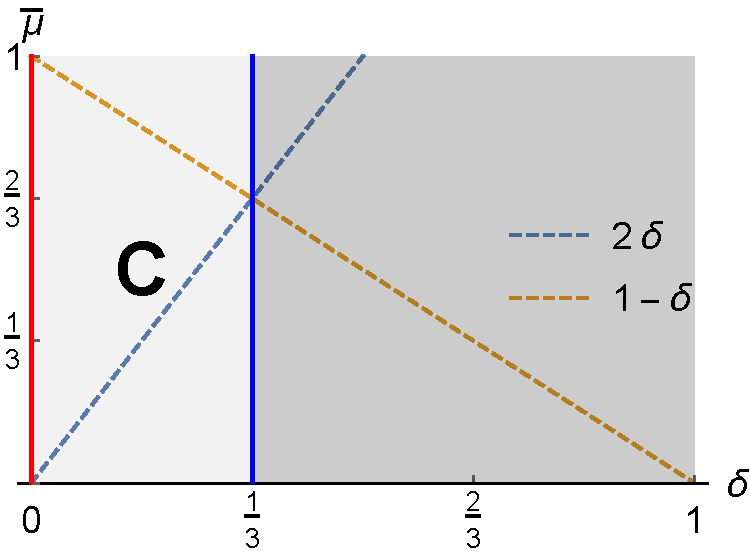
\includegraphics[scale=0.5]{prop_letter_ajhs_referee_response_nb}
\par\end{centering}
\caption{\label{fignoname}The region to the left of the vertical line at $\delta=\frac{1}{3}$
is where we assume small measurement degradation; in that region,
our extension of the KS theorem demonstrates contextuality (\textsf{C}).
In the region to the right, the degradation of the data is large,
and our extension of the KS theorem no longer refutes other explanations
for the experimental data.}
\end{figure}
The bound $\delta<\frac{1}{3}$ is tight as it is possible to construct
a $\frac{1}{3}$-deterministic QIVPM $\bar{\mu}\colon\events\rightarrow\mathscr{I}$.
For example, $\bar{\mu}_{2}'$ defined in Table~\ref{tab:probability-measures}
is a valid $\frac{1}{3}$-deterministic QIVPM\@. When $\delta\geq\frac{1}{3}$,
i.e., when the uncertainty in measurements becomes so large, it becomes
possible to map every observable to some (quite inaccurate) probability
interval, thus invalidating the Kochen-Specker theorem. We can summarize
and illustrate the above arguments using Fig.~\ref{fignoname}.

As is the case for conventional, infinitely-precise, quantum probability
measures, the theorem is only applicable to dimensions $D\geq3$.
Indeed, when the Hilbert space has dimension 2, it is straightforward
to construct a 0-deterministic QIVPM as follows. Consider a non-contextual
hidden variable model for $D=2$ (e.g., as proposed by Bell or Kochen-Specker~\cite{BELL_1966,kochenspecker1967}).
Such a two-dimen\-sional model always assigns definite values to
all observables and hence assigns a \emph{determinate} probability
(0 or 1) to each event. This probability measure directly induces
a 0-deterministic QIVPM by changing 0 to $\imposs$ and 1 to $\necess$.
It follows that every 0-deterministic QIVPM is $\delta$-deterministic.

\subsection{Experimental Data and $\delta$-determinism}

We have thus quantified one important aspect of uncertainty in quantum
mechanics---the effect of the imprecise nature of devices---which
is a novel addition to the theory of measurement. Indeed, as Heisenberg
emphasized in his famous microscope example~\cite{Heisenberg1983},
the conventional theory of measurement states that it is impossible
to precisely measure any property of a system without disturbing it
somewhat. Thus, there are fundamental limits to what one can measure
and these limits have traditionally been attributed to complementarity.
Our imprecision represents an \emph{additional} source of indeterminacy
beyond the inherent probabilistic nature of quantum mechanics.

In an experimental setup, $\delta$ is calculated as follows. To determine
the probability of any event, we typically repeat an experiment $m$
times and count the number of times we witness the event. This assumes
that for each run of the experiment we can determine, using our apparatus,
whether the event occurred or not. Assume an event has an ideal mathematical
probability of $0$, and we repeat the experiment $100$ times. In
a perfect world, we should be able to refute the event $100$ times
and calculate that the probability is $0$. We might also observe
the event $2$ times and refute it $98$ times and therefore calculate
the probability to be $0.02$. Note that this situation assumes perfect
measurement conditions and remains within the context of conventional
(real-valued) probability theory. The question we focus on is what
happens if we are only able to refute it $97$ times and are \emph{uncertain}
$3$ times? This is quite common in actual experiments. Mathematically
we can model this idea by stating that the probability of the event
is in the range $\left[0,0.03\right]$ which says that the probability
of the event could be $0$, $0.01$, $0.02$, or $0.03$ as each the
three uncertain records could either be evidence for the event or
against it. We just cannot nail it down given the current experimental
results and therefore represent the evidence as a ($\delta=$)$0.03$-deterministic
probability measure. The interesting observation is that the axioms
of probability theory (like additivity and convexity) impose enough
constraints on the structure of interval-valued quantum probability
measures to make them robust in the face of small non-vanishing $\delta$'s.

To see this idea in the context of a quantum experiment, consider
a three-dimen\-sional Hilbert space with one-dimen\-sional projectors~$P_{\rho}$,
two-dimen\-sional projectors $P_{\rho}+P_{\sigma}$, and an experiment
that is repeated $12$ times. By the Kochen-Specker theorem, it is
impossible to build a probability measure that maps every projection
to either $0=\frac{0}{12}$ or $1=\frac{12}{12}$. That is, the assignment~$\bar{\mu}_{0}$
defined in Table~\ref{tab:probability-measures} is not a QIVPM\@.

Now consider what happens if $\frac{1}{4}$ of the data for \emph{every}
one-dimen\-sional projector is uncertain. A potential account of
this degradation is to assign to each event $P$ the entire range
of possibilities $\bar{\mu}_{1}(P)$ as defined in Table~\ref{tab:probability-measures}.
This measure is not a valid QIVPM because it does not satisfy the
convexity condition: for any two orthogonal one-dimen\-sional events
$P_{0}$ and $P_{1}$, the convexity condition requires $\bar{\mu}_{1}\left(P_{0}+P_{1}\right)\subseteq\bar{\mu}_{1}\left(P_{0}\right)+\bar{\mu}_{1}\left(P_{1}\right)$,
but $\bar{\mu}_{1}\left(P_{0}+P_{1}\right)=\left[\tfrac{3}{4},1\right]$
which is not a subset of $\left[0,\tfrac{1}{2}\right]=\bar{\mu}_{1}\left(P_{0}\right)+\bar{\mu}_{1}\left(P_{1}\right)$.
Interestingly, it is impossible to find any probability measure that
would be consistent with these observations, as the interval $\left[\tfrac{3}{4},1\right]$
is completely disjoint from the interval $\left[0,\tfrac{1}{2}\right]$
and no amount of shifting of assumptions regarding the precise outcome
of the uncertain observations could change that disjointness. However,
as shown next, a sharp transition occurs when $\delta=\tfrac{1}{3}$.

When the proportion of uncertain data reaches $\frac{1}{3}$, the
probability measure that assigns to each event the entire range of
possibilities is $\bar{\mu}_{2}$ defined in Table~\ref{tab:probability-measures}.
This is also not a valid probability measure by the same argument
as above. However, in this case, $\bar{\mu}_{2}\left(P_{0}+P_{1}\right)=\left[\tfrac{2}{3},1\right]$
and $\left[0,\tfrac{2}{3}\right]=\bar{\mu}_{2}\left(P_{0}\right)+\bar{\mu}_{2}\left(P_{1}\right)$
have a \emph{common point}. Hence, by assuming that the uncertain
data for one-dimen\-sional projectors always support the associated
event, while those for two-dimen\-sional projectors always refute
the event, we can find the probability measure~$\bar{\mu}_{2}'$
that can be verified as a valid QIVPM and is consistent with the experimental
data.

A similar situation happens when more than $\frac{1}{3}$ of data
is uncertain. In particular, if half of the data is uncertain, the
probability measure~$\bar{\mu}_{3}$ that assigns to each event the
entire range of possibilities is already a QIVPM\@.

%%%%%%%%%%%%%%%%%%%%%%%%%%%%%%%%%%%%%%%%%%%%%%%%%%%%%%%%%%%%%%%%%%%


\section{The Born Rule and Gleason's Theorem\label{sec:Gleason}}

A conventional quantum probability measure can be easily constructed
from a state $\rho$ according to the Born rule \cite{Born1983,Mermin2007,Jaeger2007}.
According to Gleason's theorem~\cite{gleason1957,Redhead1987-REDINA,peres1995quantum},
this state $\rho$ is also the unique state consistent with any possible
probability measure.

\subsection{Finite-Precision Extension of Gleason's Theorem\label{subsec:Finite-Precision-Extension-of}}

In order to re-examine these results in our framework, we first reformulate
Gleason's theorem in QIVPMs using infinitely precise uncountable intervals~$\mathscr{I}_{\infty}=\set{\left[x,x\right]}{x\in\left[0,1\right]}$:

\begin{thm}[$\mathscr{I}_{\infty}$ Variant of the Gleason Theorem]\label{cor:Gleason's-1}In
a Hilbert space $\Hilb$ of dimension $D\geq3$, given a QIVPM~$\bar{\mu}\colon\events\rightarrow\mathscr{I}_{\infty}$,
the state $\rho$ consistent with~$\bar{\mu}$ on every projector
is unique, i.e., there exists a unique state~$\rho$ such that $\coreBorn\left(\bar{\mu},\events\right)=\{\rho\}$.
\end{thm}

Now let us consider relaxing $\mathscr{I}$ to a countable set of
finite-width intervals. As the intervals in the image of a QIVPM become
less and less sharp, we expect more and more states to be consistent
with it. In the limit of minimal sharpness, all states~$\rho$ are
consistent with the QIVPM 
\begin{equation}
\bar{\mu}\left(P\right)=\begin{cases}
\imposs & \textrm{ if }P=\mathbb{0}\,;\\
\necess & \textrm{ if }P=\mathbb{1}\,;\\
\unknown=\left[0,1\right] & \textrm{ otherwise}
\end{cases}
\end{equation}
mapping nearly all projections to the \emph{unknown} interval~\unknown.
There is however a subtlety: as we will show in Thm.~\ref{thm:Non-extensible-of-Gleason's}
later, it is possible for an arbitrary assignment of intervals to
projectors to be globally inconsistent, % \noindent For general QIVPMs mapping to imprecise intervals, we also
% want to seek a simple rule to construct them, and to understand which
% states are consistent with them. However, if measurement intervals are
% too imprecise, the state consistent with the results of measurements
% on some projectors might contradict the state induced by some other
% projectors. Indeed we can formally prove that, in general, there may
% be \emph{no} state consistent with some arbitrary QIVPM.
but before proving Thm.~\ref{thm:Non-extensible-of-Gleason's}, we
need the other two lemmas to simplify the proof of the convexity condition
again.

\begin{lemma}\label{thm:convex-3}Given a Hilbert space~$\Hilb$
of dimension~$3$, to verify $\bar{\mu}\colon\events\rightarrow\mathscr{I}$
is a QIVPM, it is sufficient to check Eqs.~(\ref{eq:QIVPM-constraints})
and 
\begin{equation}
\bar{\mu}\left(P'+P''\right)\subseteq\bar{\mu}\left(P'\right)+\bar{\mu}\left(P''\right)\label{amr-1}
\end{equation}
for each pair of orthogonal projectors $P'$ and~$P''$.\end{lemma}

\begin{proof}The most important part of the proof is to verify the
convexity condition for $\bar{\mu}$. Given a pair of commuting projectors
$P_{0}$ and $P_{1}$ on a three-dimen\-sional Hilbert space, they
can be diagonalized by a common orthonormal basis $\Omega=\{\ket{0},\ket{1},\ket{2}\}$.
Consider the function $\varphi\colon2^{\Omega}\rightarrow\events$
defined in Eq.~(\ref{eq:pullback-function}), there are two sets
of basis vectors $E_{0}$ and $E_{1}\subseteq\Omega$, such that $\varphi\left(E_{0}\right)=P_{0}$
and $\varphi\left(E_{1}\right)=P_{1}$. Since $E_{0}$ and $E_{1}$
are both subsets of a three-element set, their relation has only three
possibilities. The first possibility is that one of them is a subset
of the other one, $E_{0}\subseteq E_{1}$ or $E_{1}\subseteq E_{0}$.
The second possibility is that they are disjoint, $E_{0}\cap E_{1}=\emptyset$.
If neither of the previous possibilities is true, i.e., they have
some intersections, but no subset relation, then $E_{0}\cap E_{1}$,
$E_{0}\backslash E_{1}$, and $E_{1}\backslash E_{0}$ are all non-empty.
Together with the fact that $\Omega$ has only three elements, they
are all singleton sets. These three possibilities are going to be
discussed as follows.
\begin{itemize}
\item When one of them is a subset of the other one, say $E_{0}\subseteq E_{1}$,
we have $P_{0}P_{1}=\varphi\left(E_{0}\cap E_{1}\right)=P_{0}$ and
$P_{0}+P_{1}-P_{0}P_{1}=P_{1}$. Thus,
\begin{equation}
\bar{\mu}\left(P_{0}+P_{1}-P_{0}P_{1}\right)+\bar{\mu}\left(P_{0}P_{1}\right)=\bar{\mu}\left(P_{1}\right)+\bar{\mu}\left(P_{0}\right)\,.
\end{equation}
\item When $E_{0}\cap E_{1}=\emptyset$, we have $P_{0}P_{1}=\varphi\left(E_{0}\cap E_{1}\right)=\mathbb{0}$
and 
\begin{equation}
\bar{\mu}\left(P_{0}+P_{1}-P_{0}P_{1}\right)+\bar{\mu}\left(P_{0}P_{1}\right)=\bar{\mu}\left(P_{0}+P_{1}\right)\subseteq\bar{\mu}\left(P_{0}\right)+\bar{\mu}\left(P_{1}\right)\label{eq:QuantumInterval-valuedProbability-Inclusion-3}
\end{equation}
by Eq.~(\ref{amr-1}).
\item When $E_{0}\cap E_{1}$, $E_{0}\backslash E_{1}$, and $E_{1}\backslash E_{0}$
are all singleton sets, say $E_{0}\backslash E_{1}=\left\{ \ket{0}\right\} $,
$E_{1}\backslash E_{0}=\left\{ \ket{1}\right\} $, and $E_{0}\cap E_{1}=\left\{ \ket{2}\right\} $,
proving an equivalent condition for the convexity condition, Eq.~(\ref{eq:QuantumInterval-valuedProbability-Inclusion}),
is easier than proving Eq.~(\ref{eq:QuantumInterval-valuedProbability-Inclusion})
directly. Since one minus an interval maps this interval to its mirror
image, and reflection preserves the subset relations, the convexity
condition holds if and only if
\begin{equation}
\necess-\bar{\mu}\left(P_{0}P_{1}\right)+\necess-\bar{\mu}\left(P_{0}+P_{1}-P_{0}P_{1}\right)\subseteq\necess-\bar{\mu}\left(P_{0}\right)+\necess-\bar{\mu}\left(P_{1}\right)
\end{equation}
which is equivalent to
\begin{equation}
\bar{\mu}\left(\mathbb{1}-P_{0}P_{1}\right)+\bar{\mu}\left(\mathbb{1}-\left(P_{0}+P_{1}-P_{0}P_{1}\right)\right)\subseteq\bar{\mu}\left(\mathbb{1}-P_{0}\right)+\bar{\mu}\left(\mathbb{1}-P_{1}\right)
\end{equation}
because of Eq.~(\ref{eq:QIVPM-complement}). The last equation holds
because we can apply Eq.~(\ref{amr-1}) on the following chain of
equations:
\begin{equation}
\begin{aligned} & \bar{\mu}\left(\mathbb{1}-P_{0}P_{1}\right)+\bar{\mu}\left(\mathbb{1}-\left(P_{0}+P_{1}-P_{0}P_{1}\right)\right)=\bar{\mu}\left(\proj{0}+\proj{1}\right)+\bar{\mu}\left(\mathbb{0}\right)\\
\subseteq{} & \bar{\mu}\left(\proj{0}\right)+\bar{\mu}\left(\proj{1}\right)=\bar{\mu}\left(\mathbb{1}-P_{0}\right)+\bar{\mu}\left(\mathbb{1}-P_{1}\right)\,.
\end{aligned}
\end{equation}
\end{itemize}
Since the convexity condition holds for all three possibilities, $\bar{\mu}$
is a QIVPM.\end{proof}

\begin{lemma}\label{thm:convex-3-1}Given a Hilbert space~$\Hilb$
of dimension~$3$, to verify $\bar{\mu}\colon\events\rightarrow\mathscr{I}$
is a QIVPM, it is sufficient to check Eqs.~(\ref{eq:QIVPM-constraints})
and 
\begin{equation}
\bar{\mu}\left(\proj{\psi'}+\proj{\psi''}\right)\subseteq\bar{\mu}\left(\proj{\psi'}\right)+\bar{\mu}\left(\proj{\psi''}\right)\label{amr-3}
\end{equation}
for each pair of orthogonal states $\ket{\psi'}$ and $\ket{\psi''}$.\end{lemma}

\begin{proof}Since any projectors can be expressed as the sum of
orthogonal one-dimen\-sional projectors, Eq.~(\ref{amr-3}) implies
Eq.~(\ref{amr-1}) by induction, and this lemma holds because of
Lemma~\ref{thm:convex-3}.\end{proof}

After we proved the lemmas, we can state and prove the theorem that
some assignment of intervals to projectors can be globally inconsistent.

\begin{thm}[Empty Cores Exist for General QIVPMs]\label{thm:Non-extensible-of-Gleason's}There
exists a Hilbert space $\Hilb$ and a QIVPM~$\bar{\mu}\colon\events\rightarrow\mathscr{I}$
such that $\coreBorn\left(\bar{\mu},\events\right)=\emptyset$.\end{thm}
%% ajh: fixed garbled statement, add $$

\begin{proof}To prove this theorem, we need to construct a QIVPM
on some Hilbert space and verify that there are no states that are
consistent (see Def.~\ref{def:Consistency}) with it on all possible
events. Assume a Hilbert space of dimension $D=3$ with orthonormal
basis $\{\ket{0},\ket{1},\ket{2}\}$, let $\ket{\ps}=\frac{\ket{0}+\ket{1}}{\sqrt{2}}$,
$\ket{\ps'}=\frac{\ket{0}+\ket{2}}{\sqrt{2}}$, and assign 
\begin{equation}
\mathscr{I}_{0}=\left\{ \necess,\imposs,\unknown\right\} \,.\label{eq:3-value-intervals}
\end{equation}
Consider the map $\bar{\mu}\colon\events\rightarrow\mathscr{I}_{0}$
defined in Table~\ref{tab:non-Born-QIVPM}. We want to prove $\bar{\mu}$
is a QIVPM\@. Since it is easy to verify $\bar{\mu}$ satisfies Eqs.~(\ref{eq:QIVPM-constraints}),
it is sufficient by Lemma~\ref{thm:convex-3-1} to verify 
\begin{equation}
\bar{\mu}\left(\proj{\psi'}+\proj{\psi''}\right)\subseteq\bar{\mu}\left(\proj{\psi'}\right)+\bar{\mu}\left(\proj{\psi''}\right)\label{amr-2}
\end{equation}
for each pair of orthogonal states $\ket{\psi'}$ and $\ket{\psi''}$.
Since $\ket{0}$, $\ket{\ps}$, and $\ket{\ps'}$ are not orthogonal
to each other, at least one of $\bar{\mu}\left(\proj{\psi'}\right)$
and $\bar{\mu}\left(\proj{\psi''}\right)$ is unknown~$\unknown$,
which implies $\unknown\subseteq\bar{\mu}\left(\proj{\psi'}\right)+\bar{\mu}\left(\proj{\psi''}\right)$.
Together with the fact that every interval in $\mathscr{I}_{0}$ is
a subset of $\unknown$, Eq.~(\ref{amr-2}) holds, and $\bar{\mu}$
is a QIVPM\@.

\begin{table}
\begin{doublespace}
\noindent \centering{}\caption{\label{tab:non-Born-QIVPM}QIVPM~$\bar{\mu}\colon\events\rightarrow\mathscr{I}_{0}$
on a Hilbert space of dimension~$D=3$. Events are listed in the
column labeled by $P$.}
\begin{tabular}{cc}
\toprule 
$P$  & $\bar{\mu}\left(P\right)$\tabularnewline
\midrule
$\mathbb{0}$, $\proj{0}$, $\proj{\ps}$, $\proj{\ps'}$  & $\imposs$\tabularnewline
$\mathbb{1}$, $\mathbb{1}-\proj{0}$, $\mathbb{1}-\proj{\ps}$, $\mathbb{1}-\proj{\ps'}$  & $\necess$\tabularnewline
All other projectors  & $\unknown$\tabularnewline
\bottomrule
\end{tabular}
\end{doublespace}
\end{table}
Next, we will prove by contradiction that $\coreBorn\left(\bar{\mu},\events\right)$
is the empty set. Suppose there is a state $\rho=\sum_{j=1}^{N}q_{j}\proj{\phi_{j}}\in\coreBorn\left(\bar{\mu},\events\right)$,
where $\sum_{j=1}^{N}q_{j}=1$ and $q_{j}>0$. Since we assumed the
core $\coreBorn\left(\bar{\mu},\events\right)$ is non-empty, so $\muB_{\rho}(P)\in\bar{\mu}(P)$,
and Table~\ref{tab:non-Born-QIVPM} tells us that $\bar{\mu}(\proj{0})=\imposs=[0,0]$,
we must conclude that $\muB_{\rho}(\proj{0})=0\in[0,0]$, and similarly
for $\proj{\ps}$ and $\proj{\ps'}$. If this is true, then $\ip{0}{\phi_{j}}=\ip{\ps}{\phi_{j}}=\ip{\ps'}{\phi_{j}}=0$
for all~$j$, and thus 
\begin{align}
\ip{1}{\phi_{j}}=\sqrt{2}\ip{\ps}{\phi_{j}}-\ip{0}{\phi_{j}}=0\,, &  & \ip{2}{\phi_{j}}=\sqrt{2}\ip{\ps'}{\phi_{j}}-\ip{0}{\phi_{j}}=0\,.
\end{align}
The above equations imply $\ket{\phi_{j}}=\ket{0}\ip{0}{\phi_{j}}+\ket{1}\ip{1}{\phi_{j}}+\ket{2}\ip{2}{\phi_{j}}=0$,
violating the assumption that $\ket{\phi_{j}}$ is a normalized state,
and thus the theorem is proved.\end{proof}

The fact that a collection of poor measurements on a quantum system
cannot reveal the underlying state is not surprising. Under certain
conditions, we can however guarantee that the uncertainty in measurements
is consistent with \emph{some} non-empty collection of quantum states.
Furthermore, we can relate the uncertainty in measurements to the
volume of quantum states such that, in the limit of infinitely precise
measurements, the volume of states collapses to a single state.

To that end, we introduce the concept of \emph{interval maps}, which
we can use to construct a consistent family of QIVPMs. An interval
map $f\colon\left[0,1\right]\rightarrow\mathscr{I}$ maps every real-valued
probability $x\in\left[0,1\right]$ to a set of intervals $f\left(x\right)=\left[\ell,r\right]$
containing $x$, where $\left[0,1\right]$ denotes the set of real-valued
probabilities (this should not be confused with the interval-valued
probability $\unknown$). We also need a notion of \emph{norm} to
quantify the uncertainty in measurements and the distance between
(pure or mixed) states. The norm of a collection of intervals $\mathscr{I}$,
$\left\Vert \mathscr{I}\right\Vert $, is defined as the maximum length
of intervals in it. The norm of a pure state $\rho=\proj{\psi}$ is
defined as usual by $\left\Vert \psi\right\Vert =\sqrt{\ip{\psi}{\psi}}$.
For any given Hermitian operator~$A$, we choose the operator norm
$\left\Vert A\right\Vert =\max_{\left\Vert \psi\right\Vert =1}\left\Vert A\ket{\psi}\right\Vert $,
which is also known as the $2$-norm or the spectral norm~\cite{RobertsVarberg1973,peres1995quantum,GolubVanLoan1996,Foucart2012}.
In fact, for any such matrix, including the density matrix~$\rho$,
this norm is the maximum absolute value of its eigenvalues. Then,
a finite-precision extension of Gleason's theorem can be stated as
follows.

\begin{thm}[Finite-Precision Extension of the Gleason Theorem]\label{thm:Finite-precision-Gleason}Let
$f\colon\left[0,1\right]\rightarrow\mathscr{I}$ be an interval map
and let the composition $f\circ\muB_{\rho}$ be a QIVPM, where $\muB_{\rho}$
is the probability measure induced by the Born rule for a given state~$\rho$.
If a state $\rho'$ is consistent with $f\circ\muB_{\rho}$ on all
events, i.e., $\rho'\in\coreBorn\left(f\circ\muB_{\rho},\events\right)$,
then the norm of their difference is bounded by $\left\Vert \mathscr{I}\right\Vert $,
i.e., $\left\Vert \rho-\rho'\right\Vert \le\left\Vert \mathscr{I}\right\Vert $.\end{thm}

\begin{proof}Given a state~$\rho'$ consistent with $f\circ\muB_{\rho}$,
we have $\muB_{\rho'}\left(\proj{\psi}\right)\in f\left(\muB_{\rho}\left(\proj{\psi}\right)\right)$
for any one-dimen\-sional projector $P=\proj{\psi}$. Since the maximum
length of the intervals in $\mathscr{I}$ is $\left\Vert \mathscr{I}\right\Vert $,
it is also the upper bound of the difference: 
\begin{equation}
\left|\muB_{\rho'}\left(\proj{\psi}\right)-\muB_{\rho}\left(\proj{\psi}\right)\right|=\left|\melem{\psi}{\rho-\rho'}{\psi}\right|\le\left\Vert \mathscr{I}\right\Vert \,.
\end{equation}
Since $\rho-\rho'$ is Hermitian, $\max_{\left\Vert \psi\right\Vert =1}\left|\melem{\psi}{\rho-\rho'}{\psi}\right|$
is the maximum absolute value of the eigenvalues of $\rho-\rho'$~\cite{544199},
and equal to $\left\Vert \rho-\rho'\right\Vert $~\cite{GolubVanLoan1996,Foucart2012}.
Hence, $\left\Vert \rho-\rho'\right\Vert \le\left\Vert \mathscr{I}\right\Vert $.\end{proof}

\subsection{Ultramodular Functions\label{subsec:Ultramodular-Functions}}

Theorem~\ref{thm:Finite-precision-Gleason} generalizes Gleason's
theorem in the sense that it accounts for a larger class of probability
measures that includes the conventional one as a limit. The theorem
is however ``special'' in the sense that it only applies to the
particular class of QIVPMs constructed by composing an interval map
with a conventional quantum probability measure. QIVPMs constructed
in this manner have some peculiar properties that we examine next.

An interval map is called \emph{ultramodular} if it satisfies the
following properties.

\begin{definition}[Ultramodular Functions]\label{def:THOS}Given
a collection of intervals $\mathscr{I}$ including $\imposs$ and
$\necess$, an interval map $\ultramodular\colon\left[0,1\right]\rightarrow\mathscr{I}$
is called ultramodular if
\begin{align}
\ultramodular(0)=\imposs\,, &  & \ultramodular(1)=\necess\,, &  & \ultramodular\left(1-x\right)=\necess-\ultramodular\left(x\right)\,,\label{eq:iota-constraints}
\end{align}
and for any three numbers~$x_{0}$, $x_{1}$, and $x_{2}\in\left[0,1\right]$
such that $y=x_{0}+x_{1}+x_{2}\in\left[0,1\right]$, we have
\begin{equation}
\ultramodular\left(y\right)+\ultramodular\left(x_{2}\right)\subseteq\ultramodular\left(x_{0}+x_{2}\right)+\ultramodular\left(x_{1}+x_{2}\right)\,.\label{eq:iota-Inclusion}
\end{equation}
\end{definition}

\noindent The first three constraints, Eqs.~(\ref{eq:iota-constraints}),
are the direct counterpart of the corresponding QIVPM constraints,
Eqs.~(\ref{eq:QIVPM-constraints}); the last condition, Eq.~(\ref{eq:iota-Inclusion}),
is the direct counterpart of the convexity conditions, Eqs.~(\ref{eq:classicalconvex})
and~(\ref{eq:QuantumInterval-valuedProbability-Inclusion}) \cite{Choquet1954,Shapley1971,NgMoYeh1997Chinese,MarinacciMontrucchio2005}.
Therefore, these conditions guarantee that for any conventional quantum
probability measure $\mu$, the composition $\ultramodular\circ\mu$
defines a valid QIVPM\@. Conversely, if for every quantum probability
measure $\mu$, it is the case that $f\circ\mu$ is a QIVPM, then
the interval map~$f$ is an ultramodular function. Formally, we have
the following result:

\begin{thm}[Equivalence of Ultramodular Functions and IVPMs]\label{thm:iota-statements}The
following three statements are equivalent: \begin{enumerate}

\item\label{enu:iota-subject-to}A function~$\ultramodular\colon\left[0,1\right]\rightarrow\mathscr{I}$
is ultramodular.

\item\label{enu:iota-mu-CIVPM}The composite function $\ultramodular\circ\mu\colon2^{\Omega}\rightarrow\mathscr{I}$
is a classical IVPM for all classical probability measures $\mu\colon2^{\Omega}\rightarrow\left[0,1\right]$.

\item\label{enu:iota-mu-QIVPM}The composite function $\ultramodular\circ\mu\colon\events\rightarrow\mathscr{I}$
is a QIVPM for all quantum probability measures $\mu\colon\events\rightarrow\left[0,1\right]$.
\end{enumerate} \end{thm}

\begin{proof}Statement~\ref{enu:iota-subject-to} implies~\ref{enu:iota-mu-CIVPM}
and~\ref{enu:iota-mu-QIVPM} as we have outlined above. Conversely,
for the quantum case, we want to show that if $\ultramodular$ is
not ultramodular, then for some quantum probability measure $\mu$,
the composite $\ultramodular\circ\mu$ might not be a QIVPM\@. Suppose
there are three particular numbers~$x_{0}$, $x_{1}$, and $x_{2}\in\left[0,1\right]$
such that $y=x_{0}+x_{1}+x_{2}\in\left[0,1\right]$, but they don't
satisfy Eq.~(\ref{eq:iota-Inclusion}). Consider the state: 
\begin{equation}
\rho=x_{0}\proj{0}+x_{1}\proj{1}+x_{2}\proj{2}+\left(1-y\right)\proj{3}\,.
\end{equation}
The induced map $\ultramodular\circ\muB_{\rho}$ constructed using
the Born rule and blurred by $\ultramodular$ fails to satisfy Eq.~(\ref{eq:QuantumInterval-valuedProbability-Inclusion})
when $P_{0}=\proj{0}+\proj{2}$ and $P_{1}=\proj{1}+\proj{2}$. In
other words, this induced map fails to be a QIVPM\@.

For the classical case, if $\ultramodular$ is not ultramodular, we
also want to find a classical probability measure $\mu\colon2^{\Omega}\rightarrow\left[0,1\right]$
such that $\ultramodular\circ\mu$ is not a classical IVPM\@. Consider
an orthonormal basis $\Omega=\{\ket{0},\ket{1},\ldots,\ket{D-1}\}$
and $\varphi\colon2^{\Omega}\rightarrow\events$ defined by Eq.~(\ref{eq:pullback-function}).
Notice that the pullback of our previous quantum probability measure
$\muB_{\rho}$, $\varphi^{*}\muB_{\rho}$, is a classical probability
measure. If we pick $\mu$ as $\varphi^{*}\muB_{\rho}$, then the
induced map $\ultramodular\circ\mu$ fails to be a classical IVPM
for the same reason as in the quantum case.\end{proof}

In other words, the essential properties of QIVPMs constructed using
interval maps can be gleaned from the properties of ultramodular functions.
The following is the most interesting property in our setting.

\begin{thm}[Range of Ultramodular Functions]\label{thm:convex-uncountable}For
any ultramodular function~$\ultramodular\colon\left[0,1\right]\rightarrow\mathscr{I}$,
either $\mathscr{I}=\mathscr{I}_{0}$ as defined in Eq.~(\ref{eq:3-value-intervals})
or $\mathscr{I}$ contains uncountably many intervals.\end{thm}

\begin{proof}Since $\ultramodular$ maps to intervals, we can decompose
it into two functions: its left-end and right-end, where $\left[\ultramodularL\left(x\right),\ultramodularR\left(x\right)\right]=\ultramodular\left(x\right)$.
By Eq.~(\ref{eq:iota-Inclusion}), the left-end function $\ultramodularL\colon\left[0,1\right]\rightarrow\left[0,1\right]$
is Wright-convex~\cite{Wright1954,RobertsVarberg1973,PecaricTong1992},
i.e., 
\begin{equation}
\ultramodularL\left(y\right)+\ultramodularL\left(x_{2}\right)\ge\ultramodularL\left(x_{0}+x_{2}\right)+\ultramodularL\left(x_{1}+x_{2}\right)
\end{equation}
for three numbers~$x_{0}$, $x_{1}$, and $x_{2}\in\left[0,1\right]$
with $y=x_{0}+x_{1}+x_{2}\in\left[0,1\right]$. Together with the
fact that $\ultramodularL$ maps to a bounded interval $\left[0,1\right]$,
the left-end function~$\ultramodularL$ must be continuous on the
unit open interval $\left(0,1\right)$~\cite{MarinacciMontrucchio2005}.
Therefore, either $\ultramodular$ maps every number in $\left(0,1\right)$
to the same interval, or the number of intervals to which $\ultramodular$
maps must be uncountable.\end{proof}

To summarize, a conventional quantum probability measure has an uncountable
range $[0,1]$. A QIVPM constructed by blurring such a conventional
quantum probability measure must also have an uncountable range of
intervals. Of course, any particular QIVPM, or any particular experiment,
will use a fixed collection of intervals appropriate for the resources
and precision of the particular experiment.

\section{Summary}

Conventional quantum theory is based on the continuum of complex numbers,
but we cannot distinguish two arbitrary complex numbers without unbounded
resources. To explore alternative versions of quantum theory incorporating
our limitation of distinguishability, two types of discrete quantum
theories were described: \emph{quantum theories and computing over
finite fields} and \emph{quantum interval-valued probability measures
(QIVPMs)}. Examining the physical and computational consequences of
such frameworks could yield new insights into not only the subtle
properties of conventional quantum theory but also the power and capacity
of quantum computing.

The theories over finite fields started with unrestricted discrete
fields (Chapter~\ref{chap:Unrestricted-Finite-Fields}) and then
advanced to a more reasonable framework based on complexifiable discrete
fields (Secs.~\ref{discretequantumtheoryI} to~\ref{discretequantumcomputingI}),
but both of them lack a notion of probability and support unnaturally
efficient deterministic quantum algorithms. A still more plausible
discrete theory with cardinal probabilities was proposed (Secs.~\ref{sec:Discrete-Quantum-Theory-(II)}
and~\ref{discretequantumcomputingII}), where conventional quantum
theory and computing emerge in a local sense, but lacking arithmetic
operations among cardinal probabilities still posed difficulty to
define expectation values. Since the axiomatic approach looked unlikely
to provide sensible real-valued probability measures over finite fields
(Sec.~\ref{sec:Toward-IVPM}), we shifted our attention to directly
embed our limitation of distinguishability into the theory to define
QIVPM.

\begin{figure}[b]
\centering{}$\xymatrix{\textrm{Classical Probability Measure}\ar[d]_{\textrm{blur probability}}\ar[rr]^{\textrm{glue events}} &  & \textrm{Quantum Probability Measure}\ar[d]^{\textrm{blur probability}}\\
\textrm{Classical IVPM}\ar[rr]_{\textrm{glue events}} &  & \textrm{QIVPM}
}
$\caption{\label{fig:commutative-diagrams}QIVPMs inherit from both quantum
probability measures and classical IVPMs.}
\end{figure}
As a natural extension of both conventional quantum probability measures
and classical interval-valued probability measures (IVPMs) illustrated
in Fig.~\ref{fig:commutative-diagrams}, QIVPMs inherit definitions
and properties from the both frameworks. While the expectation values
with respect to QIVPMs can be pulled back to the classical ones and
consistent with those with respect to quantum probability measures
in the infinitely precise limit (Sec.~\ref{sec:Interval-Uncertainty}),
foundational concepts in quantum mechanics, such as the Kochen-Specker
and Gleason theorems, extended to QIVPMs in subtle ways. By carefully
specifying experimental uncertainties, we established rigorous bounds
on the validity of the Kochen-Specker theorem (Sec.~\ref{sec:Kochen-Specker}).
While there is a QIVPM not consistent with Gleason's unique state~$\rho$
on all projectors, we constructed a class of QIVPMs for which the
original Gleason theorem could be recovered asymptotically (Sec.~\ref{sec:Gleason}).

In the following further discussion, we will briefly explain why we
only recovered Gleason's theorem on a class of QIVPMs, the possibility
to further build a computational model over QIVPMs, and the possibility
combining both approaches to consider QIVPMs over finite fields.

\section{Gleason's Theorem for General QIVPMs}

\begin{comment}
When people proved the original Gleason theorem, people usually exploited
the geometrical structure of real 3-dimen\-sional Hilbert space \cite{gleason1957,peres1995quantum,RichmanBridges1999,Hamhalter2013}.
Since our finite-precision extension of the Gleason theorem only applies
on a class of QIVPMs, we might want to ask how to modify these geometrical
arguments to have a Gleason-type theorem for general QIVPMs. We will
further study the tensor product structure among QIVPMs which is essential
for defining product and entangled states and serves the basis to
discuss quantum nonlocality~\cite{Bell1964,Redhead1987-REDINA,peres1995quantum,Jaeger2007}
and quantum computing with QIVPMs. Finally, we want to improve the
discrete quantum theories to consider QIVPMs over finite fields in
future research.
\end{comment}
As we discussed in Sec.~\ref{sec:Gleason}, Thm.~\ref{thm:Finite-precision-Gleason}
only applies to the QIVPMs constructed by composing an interval map
with a conventional quantum probability measure, and the states consistent
with the composite QIVPM collapse to a single state as the maximum
length of intervals in $\mathscr{I}$, $\left\Vert \mathscr{I}\right\Vert $,
shrinks to $0$. In contrast, the globally inconsistent QIVPM defined
in Table~\ref{tab:non-Born-QIVPM} has the least sharp range~$\mathscr{I}_{0}$
with $\left\Vert \mathscr{I}_{0}\right\Vert =1$. This suggests a
possibility that shrinking the length $\left\Vert \mathscr{I}\right\Vert $
might help to regularize general QIVPMs, and it is natural to ask
whether there is a short enough length~$\varepsilon$ such that QIVPMs
mapping to intervals not longer than $\varepsilon$ always have non-empty
cores.

\begin{question}\label{question:approximation-Gleason}Given a Hilbert
space $\Hilb$ of dimension $D\geq3$, is there an $\varepsilon>0$
such that for all QIVPM $\bar{\mu}\colon\events\rightarrow\mathscr{I}$
satisfying $\left\Vert \mathscr{I}\right\Vert \le\varepsilon$, $\bar{\mu}$
must have a non-empty core, i.e., $\coreBorn\left(\bar{\mu},\events\right)\ne\emptyset$
?\end{question}

\begin{comment}
\todo{Discrete \foreignlanguage{ngerman}{Schrödinger} equation? And
its relationship with Grover's algorithm? }\todo{Notice that in
differential geometry, the Killing-Hopf theorem asserts that having
positive constant curvature guarantees a manifold is essentially a
sphere, but say little things even if the curvature has an only small
deviation from constant. Since a quantum probability measure is glued
by classical probability measures, like a manifold. When their relations
are exact, Gleason's theorem asserts that a quantum probability measure
can be essentially induced by the Born rule, but they can be wild
when we move on to the interval-valued situation! }
\end{comment}
To better understand this question, consider the $D=3$ situation,
where any two-dimen\-sional projectors can be expressed as the complement
of a one-dimen\-sional projector, and by Eq.~(\ref{eq:QIVPM-complement})
so does their interval-valued probabilities, i.e., 
\begin{equation}
\bar{\mu}\left(\mathbb{1}-\proj{\psi}\right)=\necess-\bar{\mu}\left(\proj{\psi}\right)\,.\label{eq:QIVPM-complement-states}
\end{equation}
Hence, a QIVPM is completely determined by its values on the one-dimen\-sional
projectors which are one-to-one corresponding to the irreducible states,
and these irreducible states are encoded in the complex projective
space $\CP{2}$ as we discussed in Sec.~\ref{subsec:Explicit-generalization-of}.
Therefore, to study a QIVPM~$\bar{\mu}$, we just need to study a
pair of functions $\frameL\colon\CP{2}\rightarrow\left[0,1\right]$
and $\frameR\colon\CP{2}\rightarrow\left[0,1\right]$ defined by $[\frameL\left(\ket{\psi}\right),\frameR\left(\ket{\psi}\right)]=\bar{\mu}\left(\proj{\psi}\right)$
for any irreducible state $\ket{\psi}\in\CP{2}$. According to Lemma~\ref{thm:convex-3-1},
$\bar{\mu}\colon\events\rightarrow\mathscr{I}$ is a QIVPM if and
only if $\bar{\mu}$ satisfies Eqs.~(\ref{eq:QIVPM-constraints})
and
\begin{equation}
\bar{\mu}\left(\mathbb{1}-\proj{\psi_{0}}\right)\subseteq\bar{\mu}\left(\proj{\psi_{1}}\right)+\bar{\mu}\left(\proj{\psi_{2}}\right)\label{eq:interval-valued-inclusion}
\end{equation}
for all orthonormal basis $\left\{ \ket{\psi_{i}}\right\} _{i=0}^{2}$
because $\proj{\psi_{1}}+\proj{\psi_{2}}=\mathbb{1}-\proj{\psi_{0}}$.
By applying Eq.~(\ref{eq:QIVPM-complement-states}) on the left-hand
side, Eq.~(\ref{eq:interval-valued-inclusion}) is equivalent to
the following interval-inclusion
\begin{eqnarray}
 &  & \necess-\left[\frameL\left(\ket{\psi_{0}}\right),\frameR\left(\ket{\psi_{0}}\right)\right]\subseteq\left[\frameL\left(\ket{\psi_{1}}\right),\frameR\left(\ket{\psi_{1}}\right)\right]+\left[\frameL\left(\ket{\psi_{2}}\right),\frameR\left(\ket{\psi_{2}}\right)\right]\label{eq:interval-valued-frame-function}\\
 & \Leftrightarrow & \left[1-\frameR\left(\ket{\psi_{0}}\right),1-\frameL\left(\ket{\psi_{0}}\right)\right]\subseteq\left[\frameL\left(\ket{\psi_{1}}\right)+\frameL\left(\ket{\psi_{2}}\right),\frameR\left(\ket{\psi_{1}}\right)+\frameR\left(\ket{\psi_{2}}\right)\right]\,.\nonumber 
\end{eqnarray}
This interval-inclusion can be rephrased as a long inequality
\begin{equation}
\frameL\left(\ket{\psi_{1}}\right)+\frameL\left(\ket{\psi_{2}}\right)\le1-\frameR\left(\ket{\psi_{0}}\right)\le1-\frameL\left(\ket{\psi_{0}}\right)\le\frameR\left(\ket{\psi_{1}}\right)+\frameR\left(\ket{\psi_{2}}\right)\,.
\end{equation}
Since $\left\Vert \mathscr{I}\right\Vert \le\varepsilon$, the length
of every interval $\left[\frameL\left(\ket{\psi}\right),\frameR\left(\ket{\psi}\right)\right]$
is bounded by $\varepsilon$ as well, which implies the largest term
in the previous inequality $\frameR\left(\ket{\psi_{1}}\right)+\frameR\left(\ket{\psi_{2}}\right)$
is bounded by $\frameL\left(\ket{\psi_{1}}\right)+\frameL\left(\ket{\psi_{2}}\right)+2\varepsilon$.
In other words, the left-end function~$\frameL$ satisfies the following
inequalities
\begin{subequations}
\begin{eqnarray}
 &  & \frameL\left(\ket{\psi_{1}}\right)+\frameL\left(\ket{\psi_{2}}\right)\le1-\frameL\left(\ket{\psi_{0}}\right)\le\frameL\left(\ket{\psi_{1}}\right)+\frameL\left(\ket{\psi_{2}}\right)+2\varepsilon\\
 & \Leftrightarrow & 1-2\varepsilon\le\sum_{i=0}^{2}\frameL\left(\ket{\psi_{i}}\right)\le1\,.\label{eq:left-end-frame-function}
\end{eqnarray}
\end{subequations}
In this language, Gleason's theorem basically states that when $\varepsilon=0$,
given any function $\frameL\colon\CP{2}\rightarrow\left[0,1\right]$
satisfying Eq.~(\ref{eq:left-end-frame-function}), there exists
a unique mixed state~$\rho$ such that 
\begin{equation}
\frameL\left(\ket{\psi}\right)=\melem{\psi}{\rho}{\psi}\label{eq:Gleason-for-CP2}
\end{equation}
for any state $\ket{\psi}\in\CP{2}$. Our Question~\ref{question:approximation-Gleason}
then ask how $\frameL$ would look like with a positive $\varepsilon$.

With different settings, whether there is an approximate version of
Gleason's theorem was asked by Sam Sanders in \emph{constructivenews}
on 2013~\cite{Sanders2013}, and there is no clear answer for his
question. To have an idea of how hard this question could be, recall
in Sec.~\ref{sec:fuzzy} we state that a quantum probability space
is glued by a family of classical probability spaces. This is like
the situation that a manifold is glued by many local coordinates.
When each small piece has \emph{exactly} the same and positive curvature,
the Killing-Hopf theorem asserts this manifold is a sphere, but little
can we say even if the curvature has a small deviation from constant.
A similar situation might happen when approximating Gleason's theorem,
but this time the whole space is glued by ``local'' classical probability
space defined by each orthonormal basis $\left\{ \ket{\psi_{i}}\right\} _{i=0}^{2}$.
When the sum of $\frameL$, $\sum_{i=0}^{2}\frameL\left(\ket{\psi_{i}}\right)$,
is \emph{exactly} the same and equal to $1$, Gleason's theorem asserts
that $\frameL$ can be expressed as Eq.~(\ref{eq:Gleason-for-CP2}).
However, when each local classical probability space becomes imprecise,
a general $\frameL$ might be as wild as we can imagine, and we might
need to know a bit more, like its QIVPM is a composite function, to
deduce its global property.

\section{And Beyond\ldots}

After we build the quantum interval-valued probability model, we might
want to know how powerful a quantum computer could be based on this
model. Since the conventional quantum circuit model manipulates the
probability amplitudes instead of the measured probabilities, either
a quantum computing model above QIVPMs needs to simultaneously manipulate
all states in the core of a QIVPM, or we need to find a way to manipulate
a QIVPM directly. However, both strategies are not straightforward.
On one hand, as we proved in Thm.~\ref{thm:Non-extensible-of-Gleason's},
a QIVPM might have an empty core which cannot be evolved over time.
On the other hand, if we want to manipulate and compute QIVPMs directly
for multi-qubit algorithms, we need to glue the QIVPM for each qubit
or subsystem together to get the QIVPM of the whole system, and this
is not straightforward either.

A successful interval-valued theory might be further extended over
finite fields based on the following definition.

\begin{definition}[Quantum Interval-valued Probability Measures
over Finite Fields]\label{def:QIVPMFF}Consider a vector space~$\mathcal{H}$
of dimension~$D$ over the complexified field~$\Fpp$, its set of
events~$\events_{p^{2}}$ as defined in Def.~\ref{def:QPMFF}, and
a collection of intervals~$\mathscr{I}$. A quantum interval-valued
probability measure over finite field $\bar{\mu}\colon\events_{p^{2}}\rightarrow\mathscr{I}$
assigns an interval to each event~$P$ subject to $\bar{\mu}(\mathbb{0})=\imposs$,
$\bar{\mu}(\mathbb{1})=\necess$, $\bar{\mu}\left(\mathbb{1}-P\right)=\necess-\bar{\mu}\left(P\right)$,
and satisfying for each pair of \emph{commuting} events~$P_{0}$
and~$P_{1}$ with $P_{0}P_{1}=P_{1}P_{0}$, 
\begin{equation}
\bar{\mu}\left(P_{0}+P_{1}-P_{0}P_{1}\right)+\bar{\mu}\left(P_{0}P_{1}\right)\subseteq\bar{\mu}\left(P_{0}\right)+\bar{\mu}\left(P_{1}\right)\,.\label{eq:QuantumInterval-valuedProbability-Inclusion-Finite-Field}
\end{equation}
\end{definition}

\noindent Understanding the properties of these probability measures
and whether we could define a ``sensible'' Born rule upon them combines
two approaches for dealing with the continuous quantities used in
the conventional quantum theory and will be the next natural extension
for our discrete quantum theories and computing.

\begin{comment}
\printbibliography
\end{comment}
\printbibliography
\end{document}
